\PassOptionsToPackage{dvipsnames}{xcolor}
\documentclass{beamer}
\usepackage[utf8]{inputenc}

\usetheme{Madrid}
\usecolortheme{default}
\useinnertheme{circles}

\definecolor{Logo1}{rgb}{0, 0.4, 0.6}
%\definecolor{Logo2}{rgb}{0.92, 0.9, 0.9}

% --- Pacotes extra ---
\usepackage{simpler-wick}
\usepackage{cancel}
\usepackage{xfrac}
\usepackage{comment}
\usepackage{dsfont}
\usepackage{amsmath}
\usepackage{amsfonts}
\usepackage{amssymb}
\usepackage{graphicx}

% cor de titulos
\setbeamercolor*{palette primary}{bg=brown!70!white, fg=white}
% cor do meio
\setbeamercolor*{palette secondary}{bg=brown!70!white, fg=white}
% cor do autor
\setbeamercolor*{palette tertiary}{bg=brown!70!white, fg=white} 
\setbeamercolor*{palette quaternary}{bg=brown!70!white,fg=white}

% cor da estrutura tipo toc, itemize...
\setbeamercolor{section in toc}{fg=brown!70!white}
\setbeamercolor{structure}{fg=red!80!black}
\setbeamercolor{itemize subitem}{fg=red!80!black}

% cor das caixas
\setbeamercolor{block title}{fg=white, bg=red!80!black}
\setbeamercolor{block body}{bg=red!10!white}

\setbeamercolor{block title alerted}{fg=white, bg=orange!95!black}
\setbeamercolor{block body alerted}{bg=orange!15!white}

\setbeamercolor{block title example}{fg=white, bg=ForestGreen!80!black}
\setbeamercolor{block body example}{bg=ForestGreen!10!white}

\setbeamertemplate{blocks}[rounded][shadow=false]

%------------------------------------------------------------
\vspace*{-2.2cm}

\title[Self-consistent Majorana nanowires]{\Large \textbf{Hybrid versus intrinsic Majorana nanowires, a self-consistent Hartree-Fock-Bogoliubov analysis} \\ \vspace*{0.5cm} \large \underline{Francisco Lobo}, Elsa Prada, Pablo SanJose}

\author[Francisco Lobo]{}

\institute[]{}

\date[ICMM-CSIC]

%------------------------------------------------------------
\begin{document} 
{\usebackgroundtemplate{

\includegraphics[width=\paperwidth,height=\paperheight]{images/assets/cover}}

\frame{\titlepage}}

%------------------------------------------------------------
{\usebackgroundtemplate{
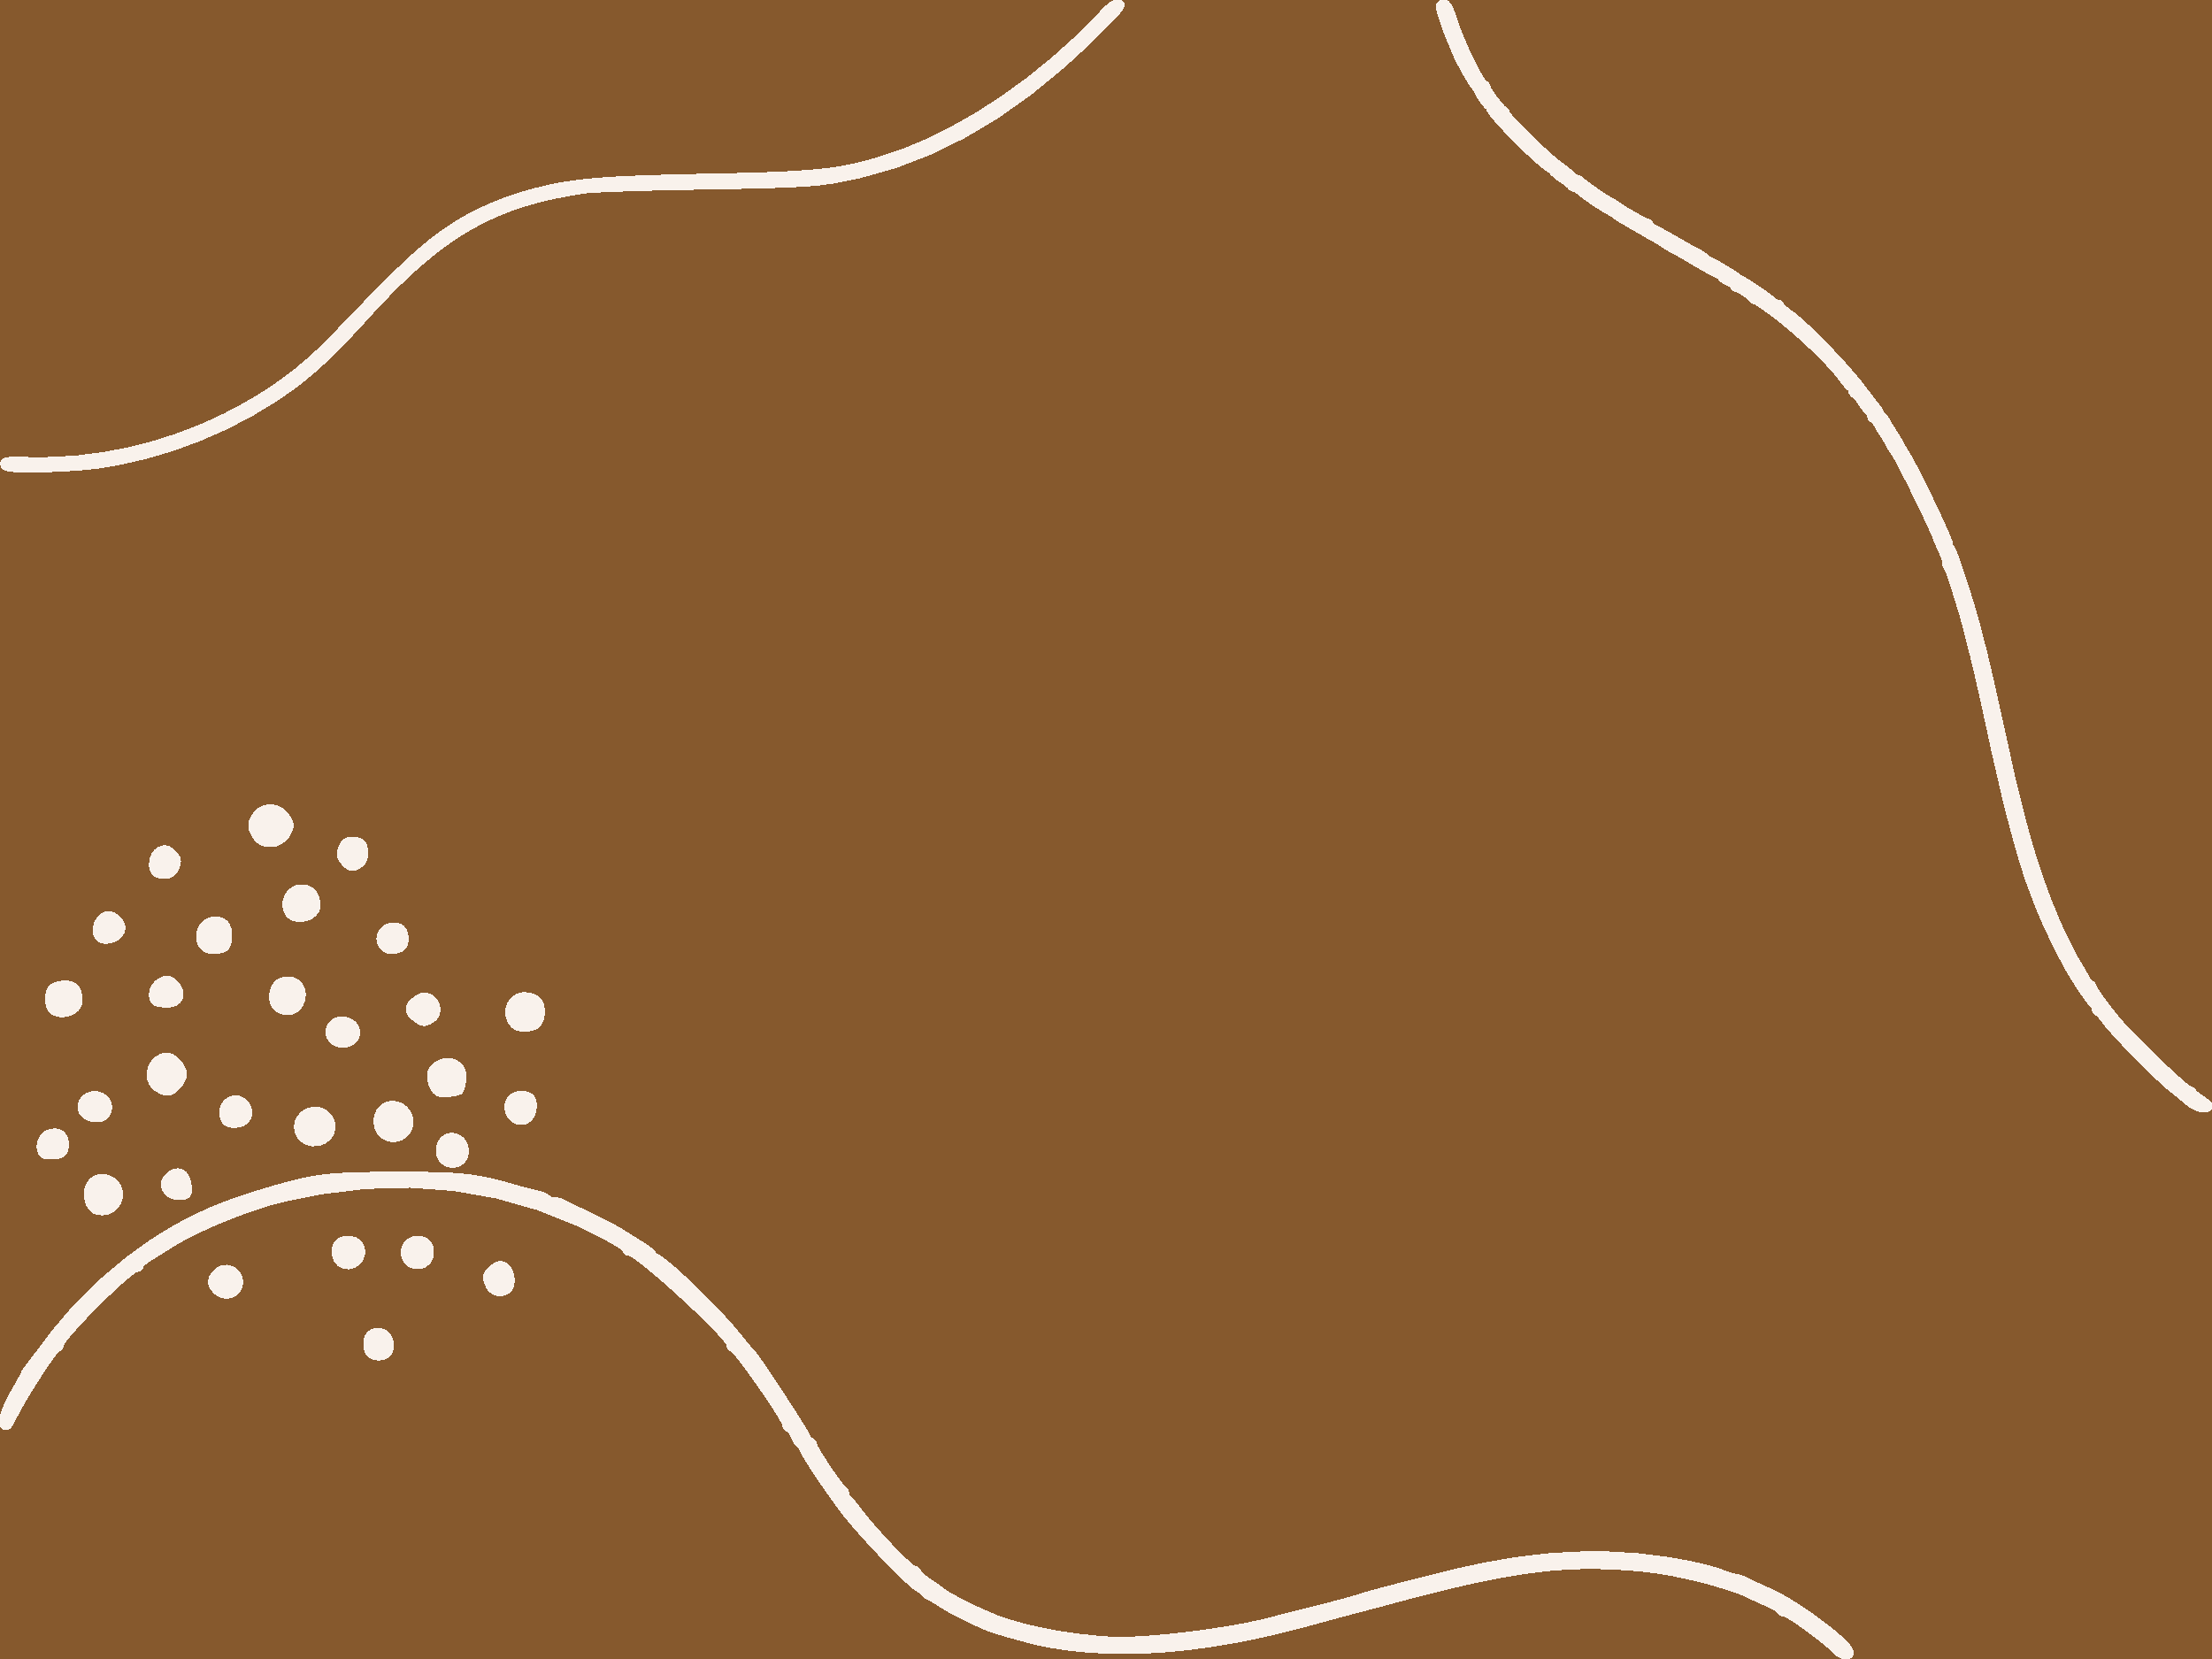
\includegraphics[width=\paperwidth,height=\paperheight]{images/assets/transition2}}
\begin{frame}[noframenumbering]

\begin{center}
\Huge \textcolor{brown!10!white}{\textbf{Index}}
\end{center}

\end{frame}}

%------------------------------------------------------------
\begin{frame}{Index}

\Large
\textcolor{red!80!black}{\textbf{\underline{Main body:}}}
\begin{enumerate}
\item Introduction
\item Oreg-Lutchyn's miminal Majorana model
\item Self-consistent HFB Majorana nanowires $^{(*)}$
\item Result of self-consistency for:
\end{enumerate}
\hspace{0.3cm} $\textcolor{red!80!black}{\bullet}$ \underline{Hybrid} nanowires (finite and infinite length)\\
\hspace{0.3cm} $\textcolor{red!80!black}{\bullet}$ \underline{Intrinsic} nanowires (finite and infinite length)

\vspace{0.3cm}
\begin{colormixin}{33!bg}
\textcolor{red!80!black}{\textbf{$^{(*)}$ \underline{Appendix:}}}
\begin{itemize}
\item Hartree-Fock-Bogoliubov mean-field theory
\item Analytical BCS gap equation accounting for Zeeman
\end{itemize}
\end{colormixin}

\end{frame}

%------------------------------------------------------------
{\usebackgroundtemplate{
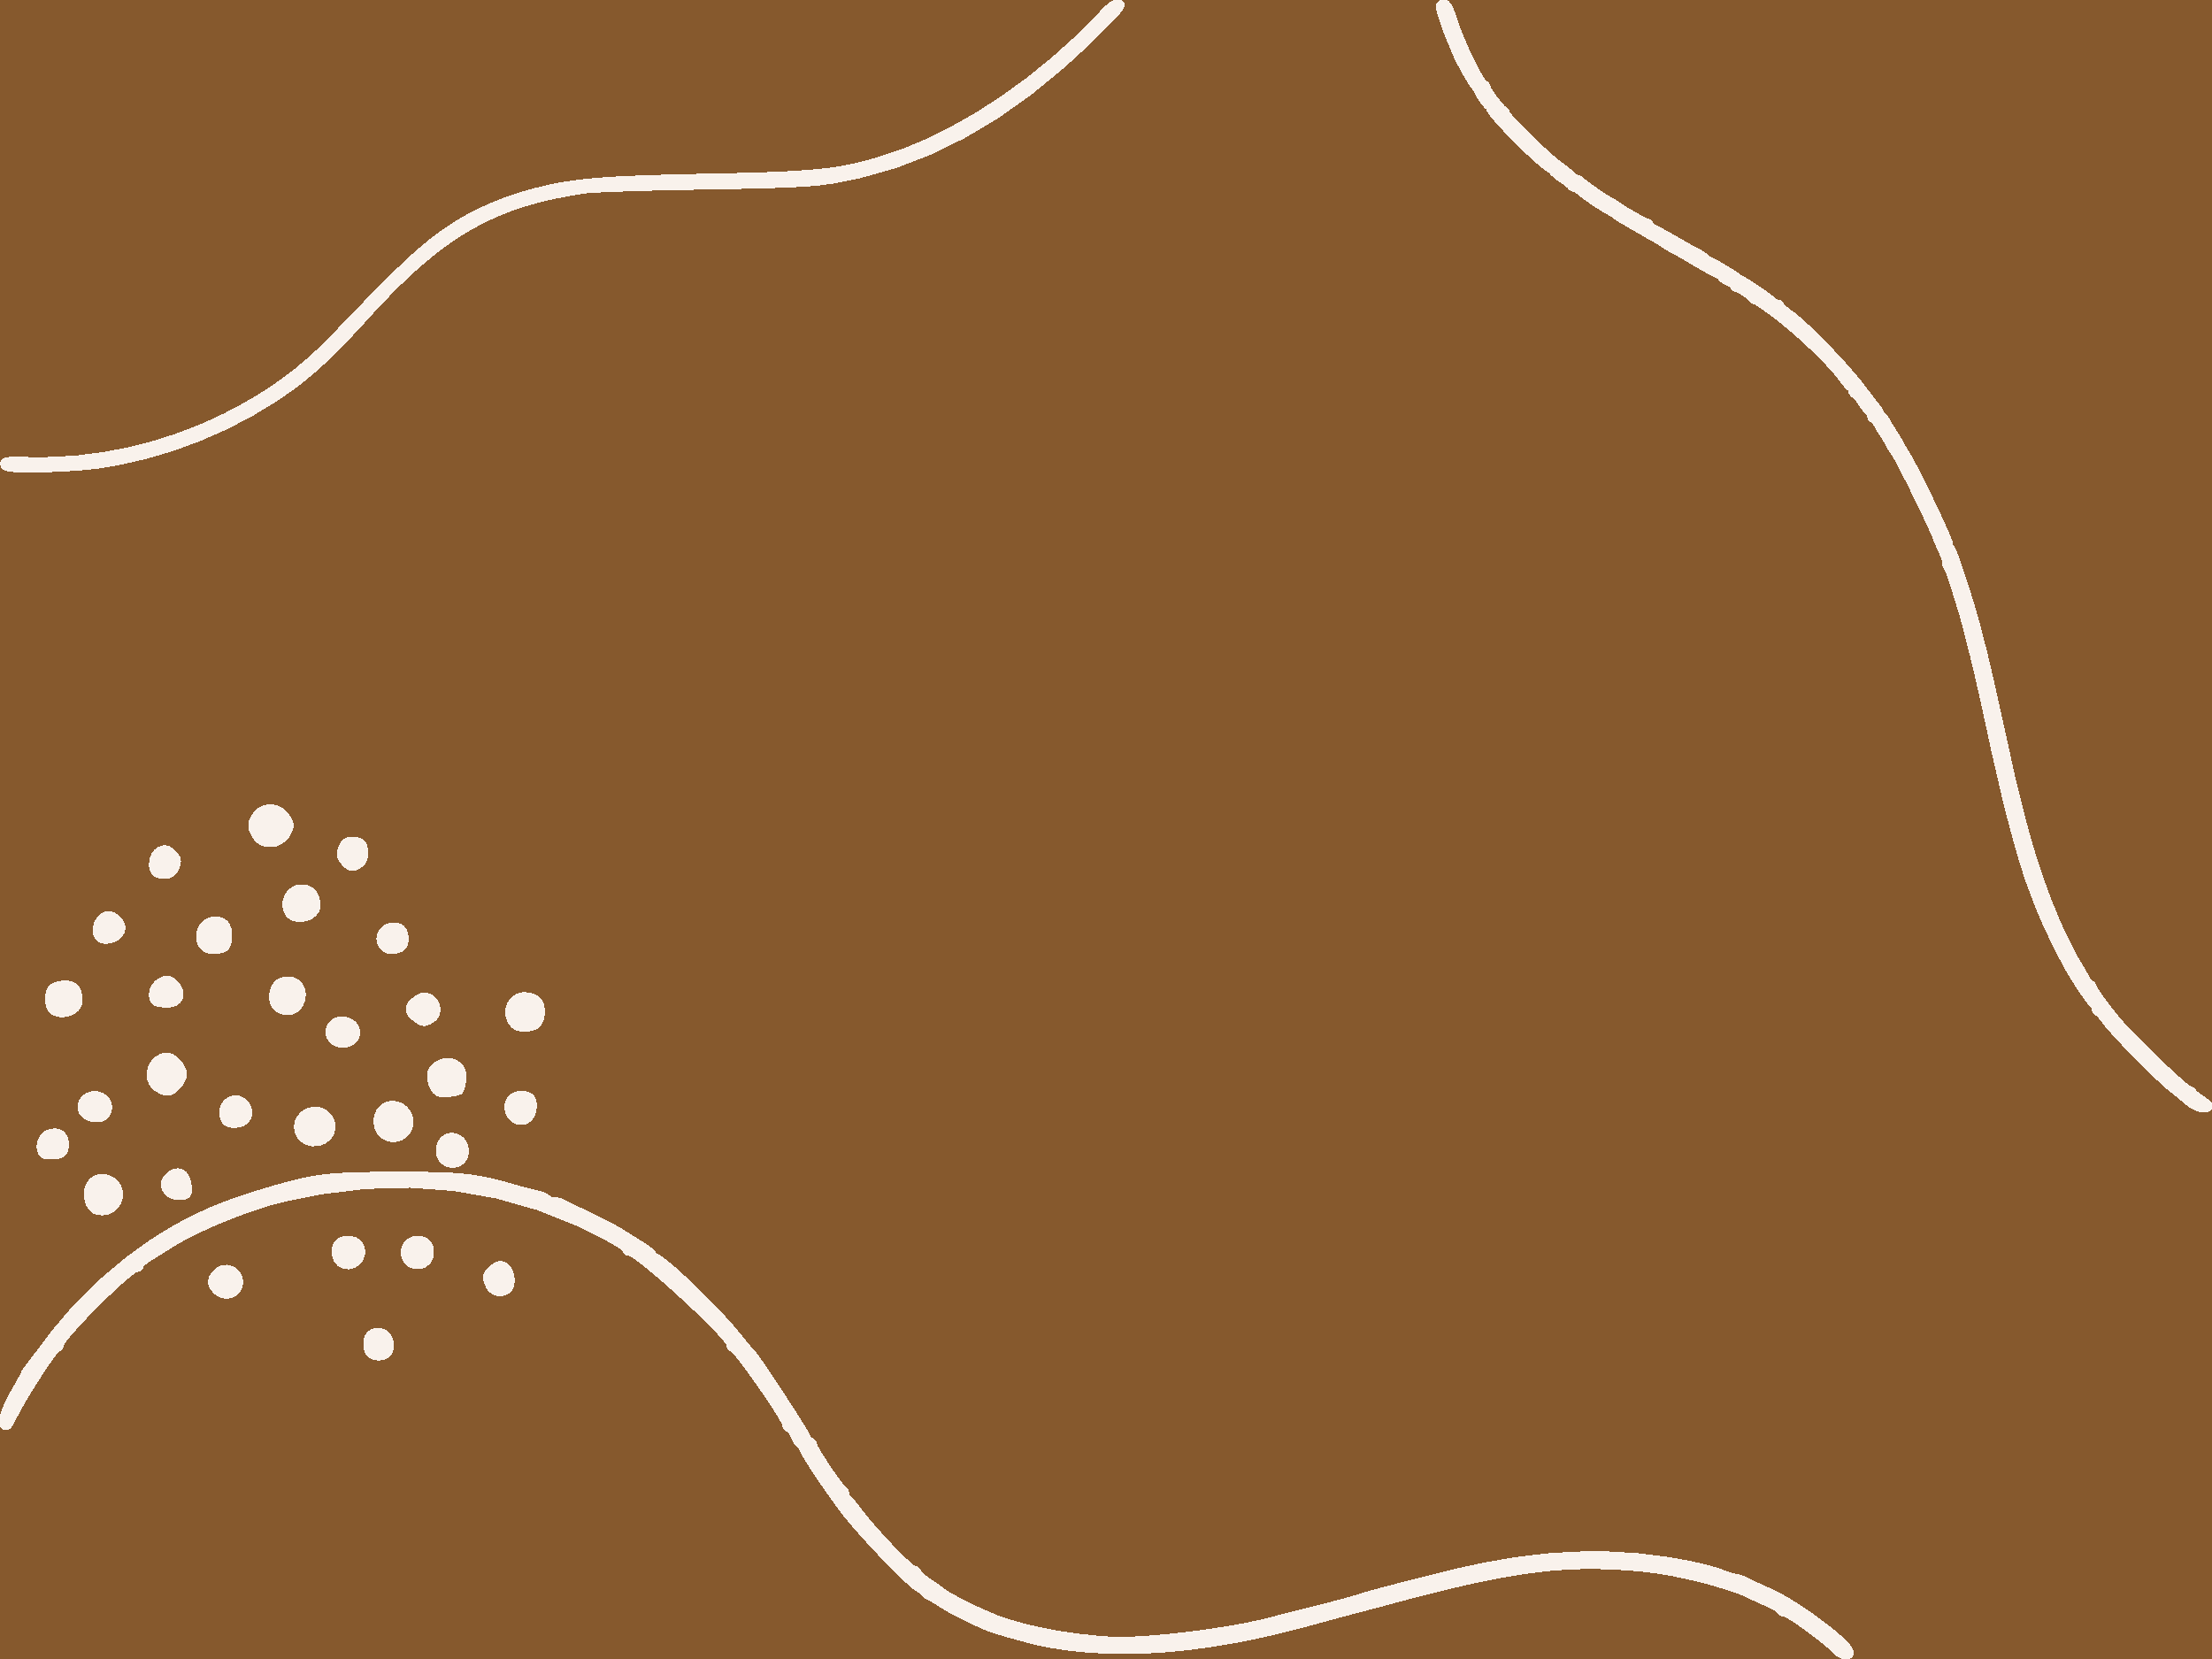
\includegraphics[width=\paperwidth,height=\paperheight]{images/assets/transition2}}
\begin{frame}[noframenumbering]

\begin{center}
\Huge \textcolor{brown!10!white}{\textbf{Main \\ body}}
\end{center}

\end{frame}}


%------------------------------------------------------------
{\usebackgroundtemplate{
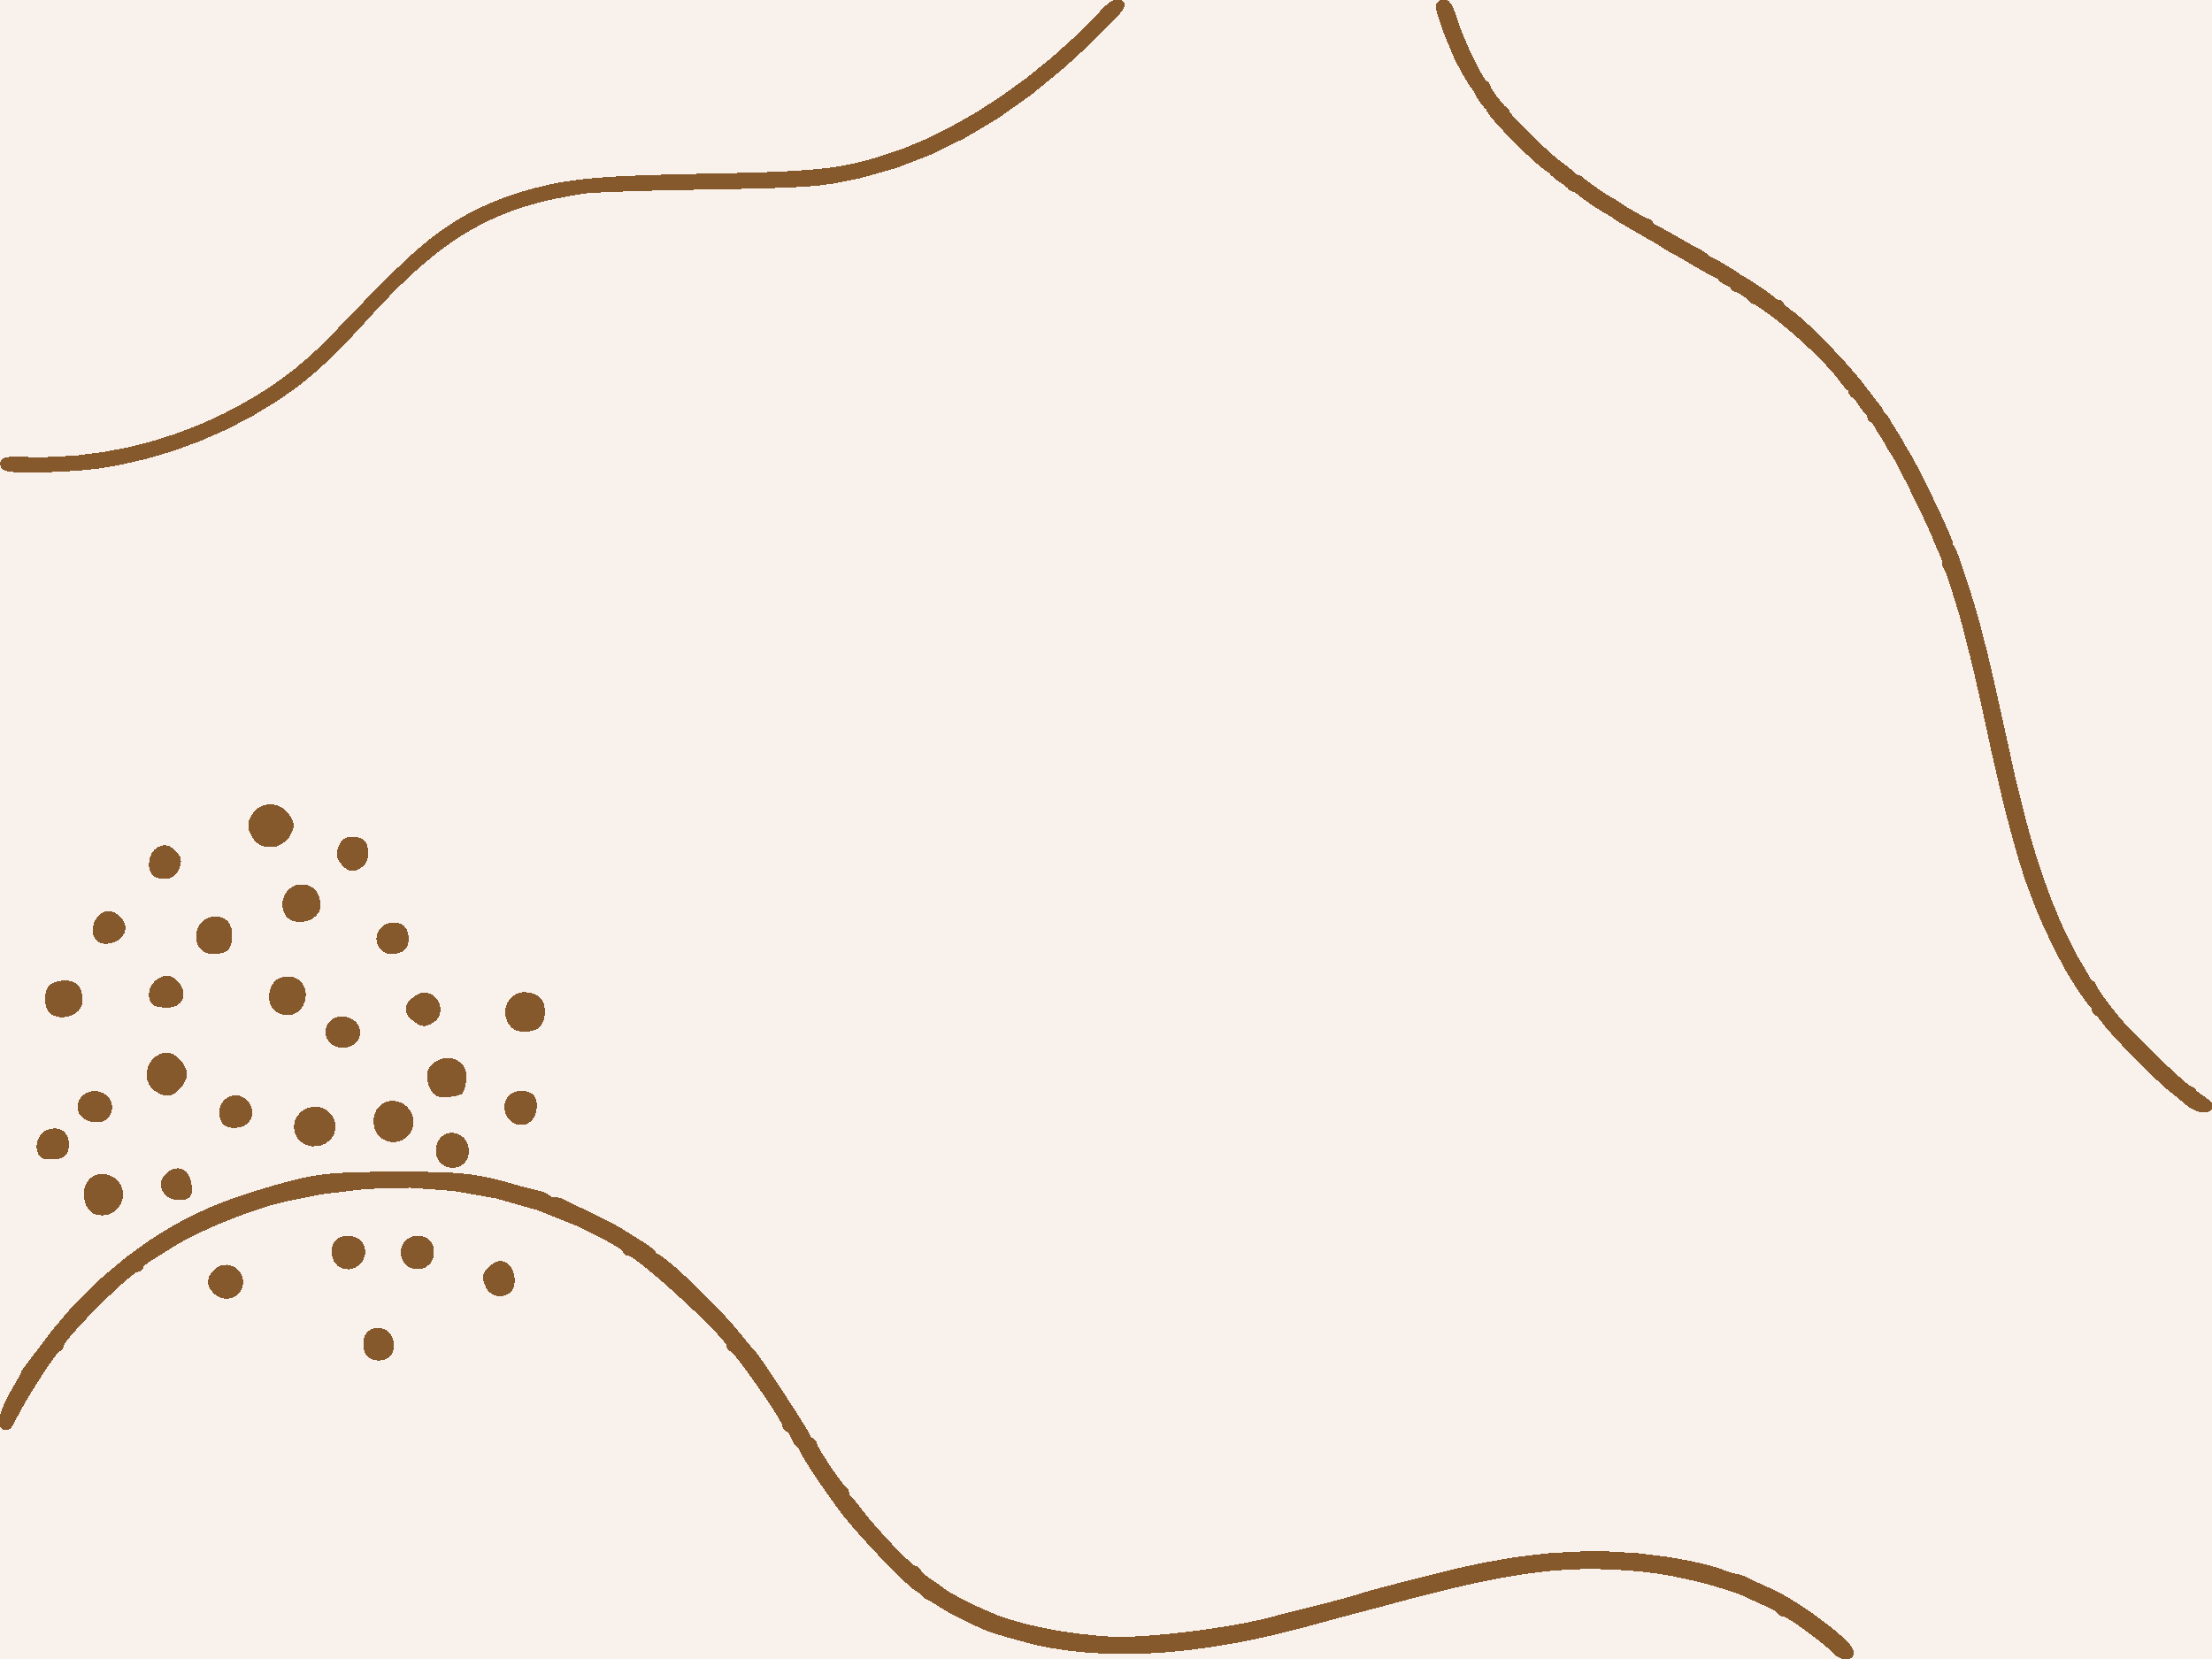
\includegraphics[width=\paperwidth,height=\paperheight]{images/assets/transition}}
\begin{frame}[noframenumbering]

\begin{center}
\Huge \textcolor{brown!70!black}{\textbf{Introduction}}
\end{center}

\end{frame}}

%------------------------------------------------------------
{\setbeamercolor{itemize item}{fg=red!80!black}
\begin{frame}{Introduction}

\textcolor{red!80!black}{\large \textbf{What are Majoranas?}}  
\textcolor{red!80!black}{$\bullet$} Zero-energy, \textcolor{red!80!black}{$\bullet$} sub-gap, \textcolor{red!80!black}{$\bullet$} boundary, \\ \textcolor{red!80!black}{$\bullet$} topologically protected, \textcolor{red!80!black}{$\bullet$} self-conjugate states of \textcolor{red!80!black}{$\bullet$} braiding statistics

\vspace*{0.2cm}
\textcolor{red!80!black}{\large 
\textbf{Why are they a hot-topic?}} \textcolor{red!80!black}{$\bullet$} Fault-tolerant qubits

\begin{center}
\begin{figure}
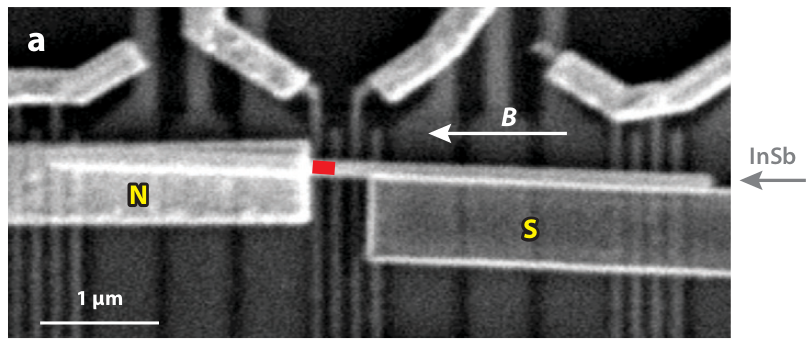
\includegraphics[scale=0.2]{images/model_exp}
\end{figure}
\end{center}

\textcolor{red!80!black}{\large \textbf{Goals:}}
Unambiguous signature of Majoranas in \textcolor{red!80!black}{hybrid} systems: \\ 
\textcolor{red!80!black}{$\bullet$} optimized proximity effect, \textcolor{red!80!black}{$\bullet$} non-invasing contacts, \textcolor{red!80!black}{$\bullet$} reduced disorder

\vspace*{0.2cm}
\textcolor{red!80!black}{\large \textbf{Solution?}}
\textcolor{red!80!black}{Intrinsic} dilluted superconductor nanowire with SOC

\end{frame}}

%------------------------------------------------------------
{\usebackgroundtemplate{
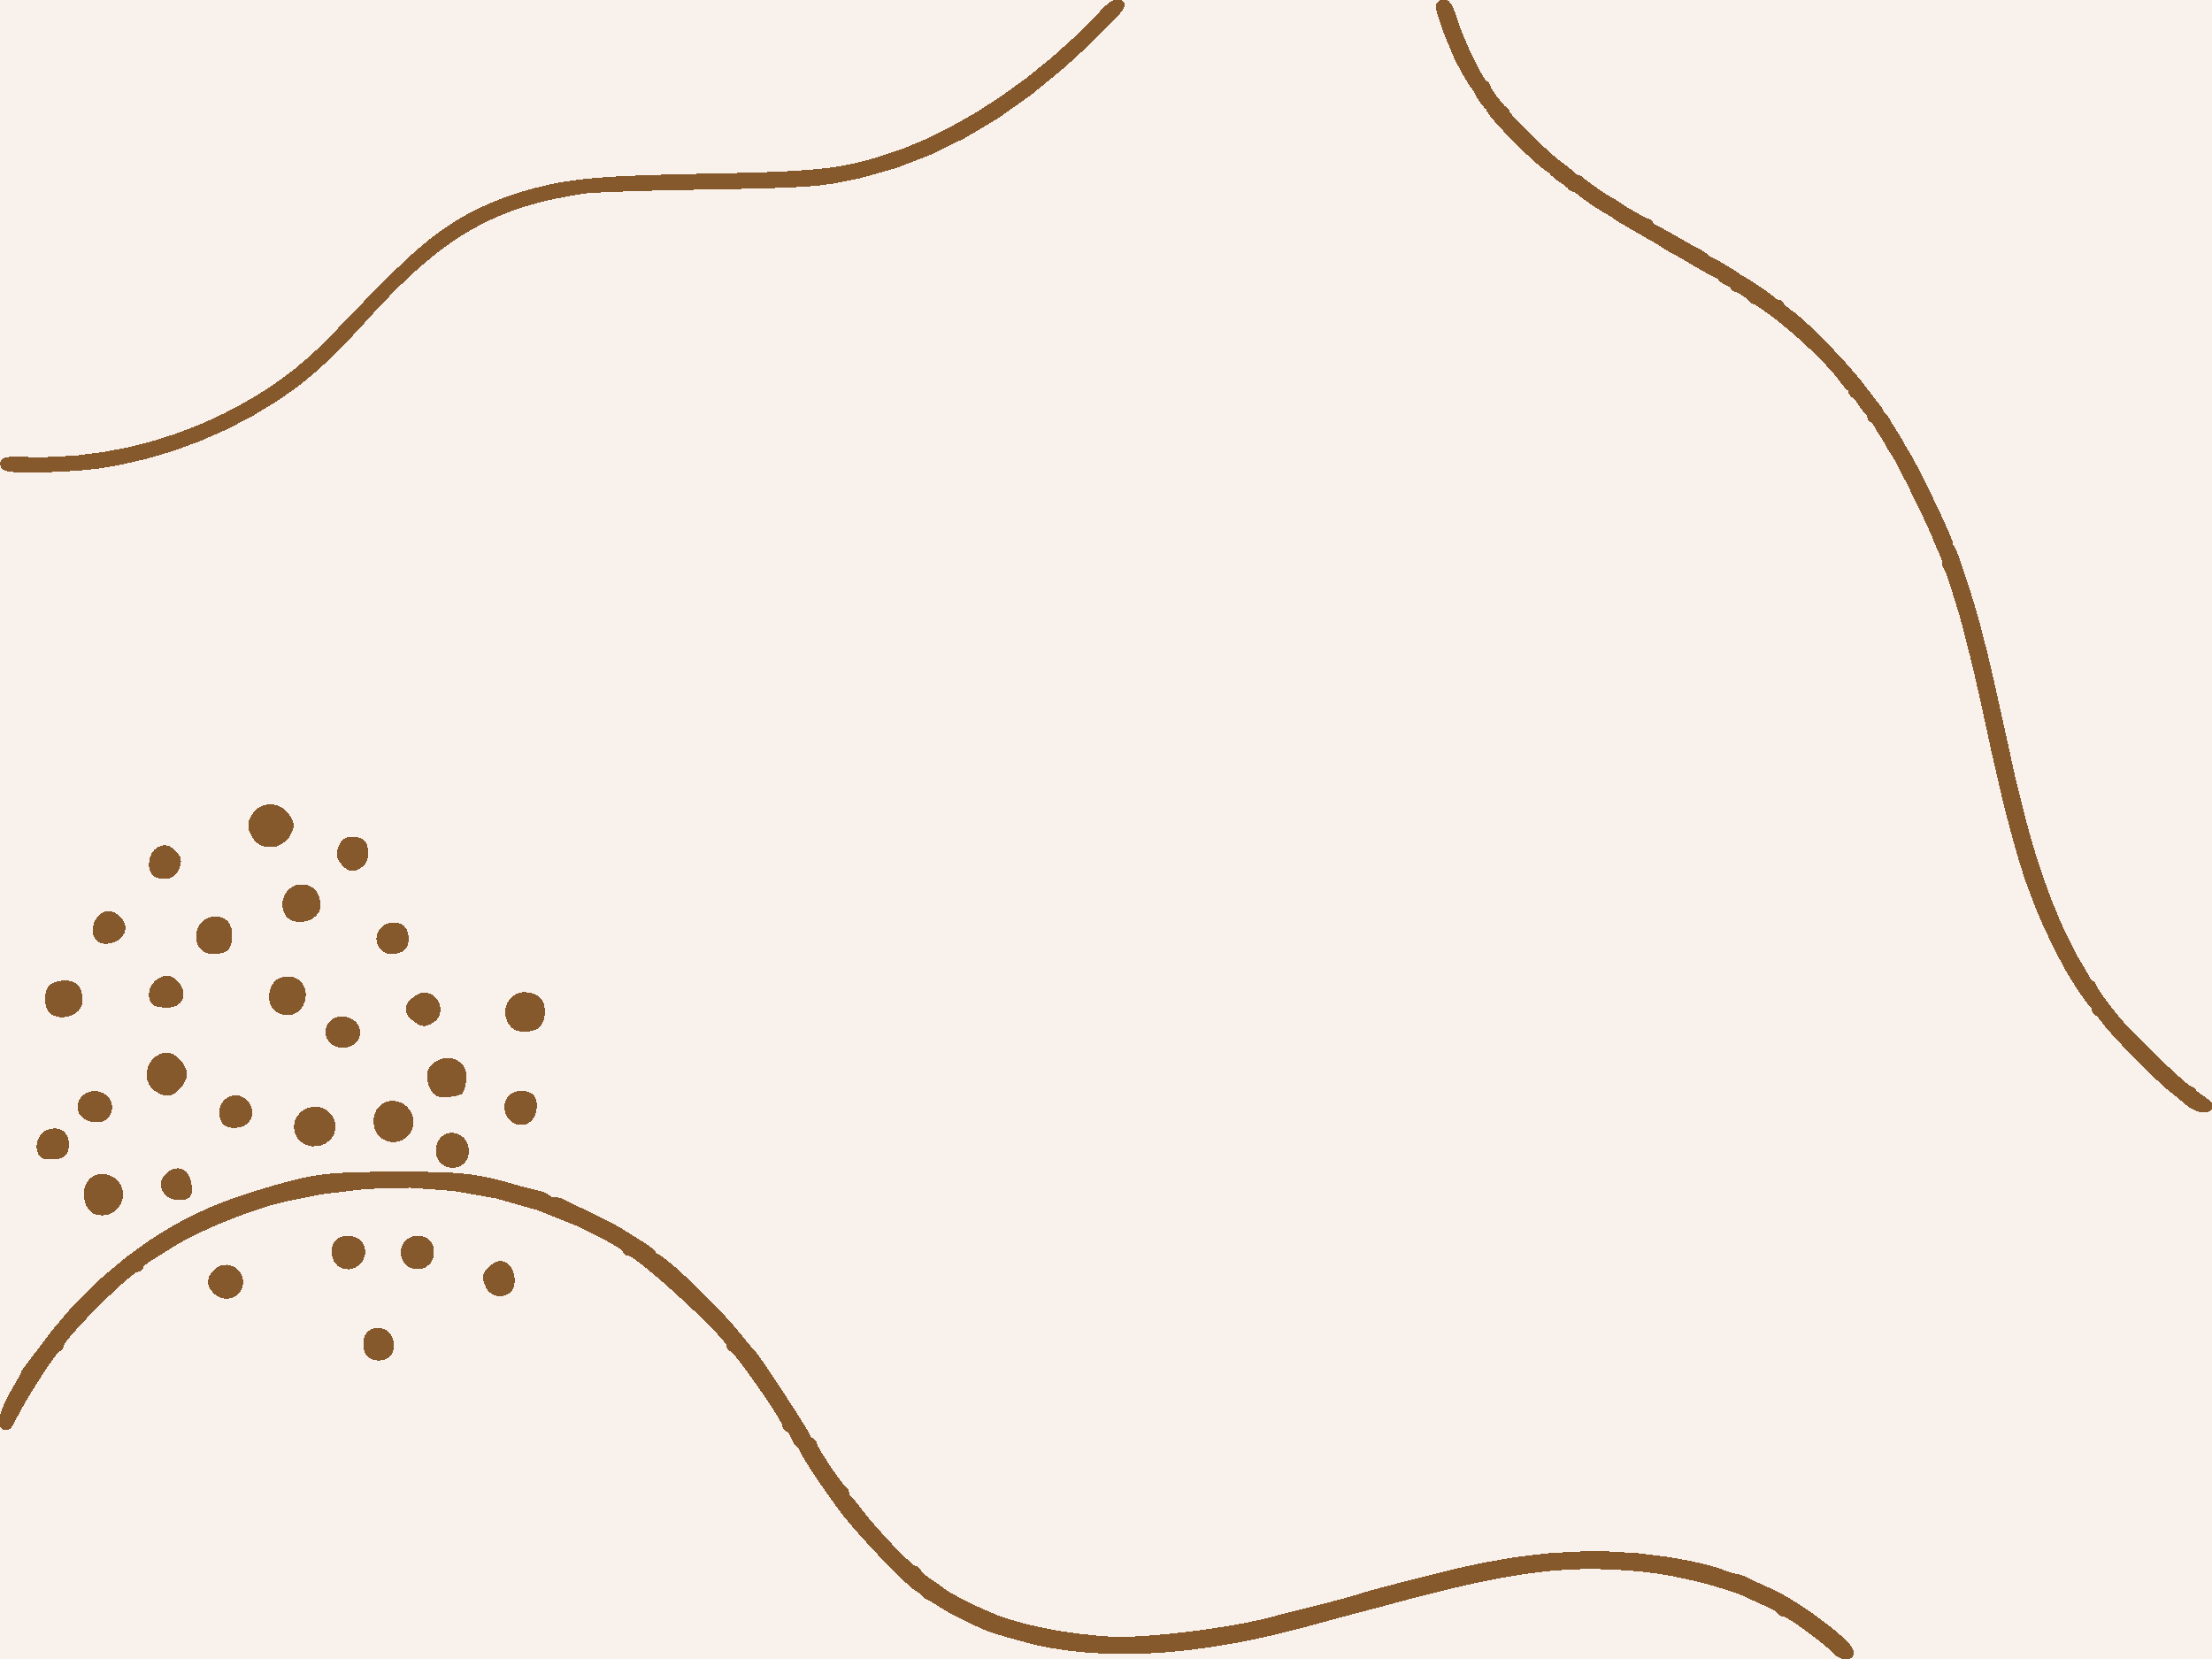
\includegraphics[width=\paperwidth,height=\paperheight]{images/assets/transition}}
\begin{frame}[noframenumbering]

\begin{center}
\Huge \textcolor{brown!70!black}{\textbf{Oreg-Lutchyn's}} \\
\Huge \textcolor{brown!70!black}{\textbf{Mininal Majorana}} \\
\Huge \textcolor{brown!70!black}{\textbf{nanowire model}} \\
\end{center}

\end{frame}}

%------------------------------------------------------------
\begin{frame}
\frametitle{Oreg-Lutchyn's Minimal Majorana model}

\vspace*{-5mm}
\begin{center}
\begin{figure}
\hspace*{-3mm}
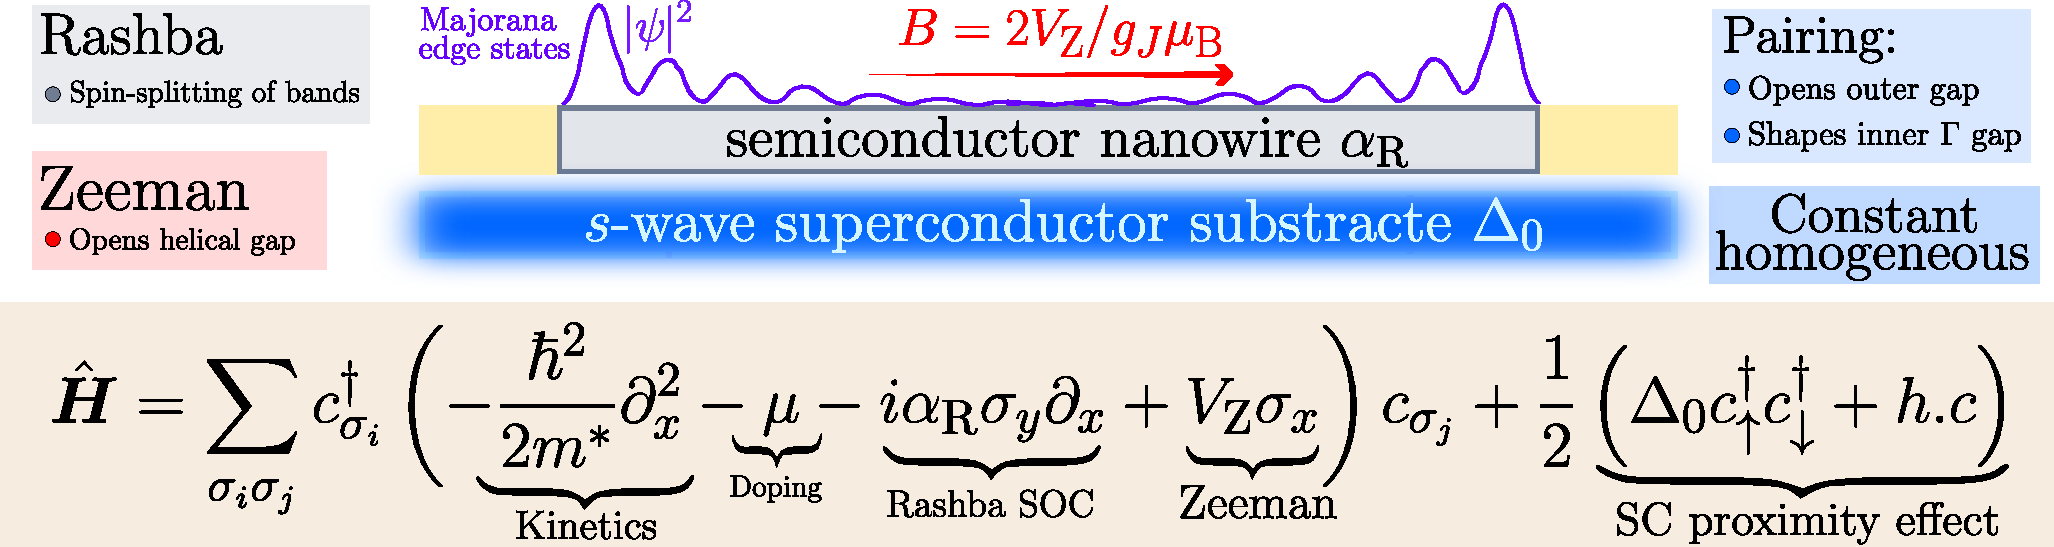
\includegraphics[scale=0.36]{images/lutchyn1}
\end{figure}
\end{center}

\pause
\vspace*{-5mm}
\begin{center}
\begin{figure}
\hspace*{-3mm}
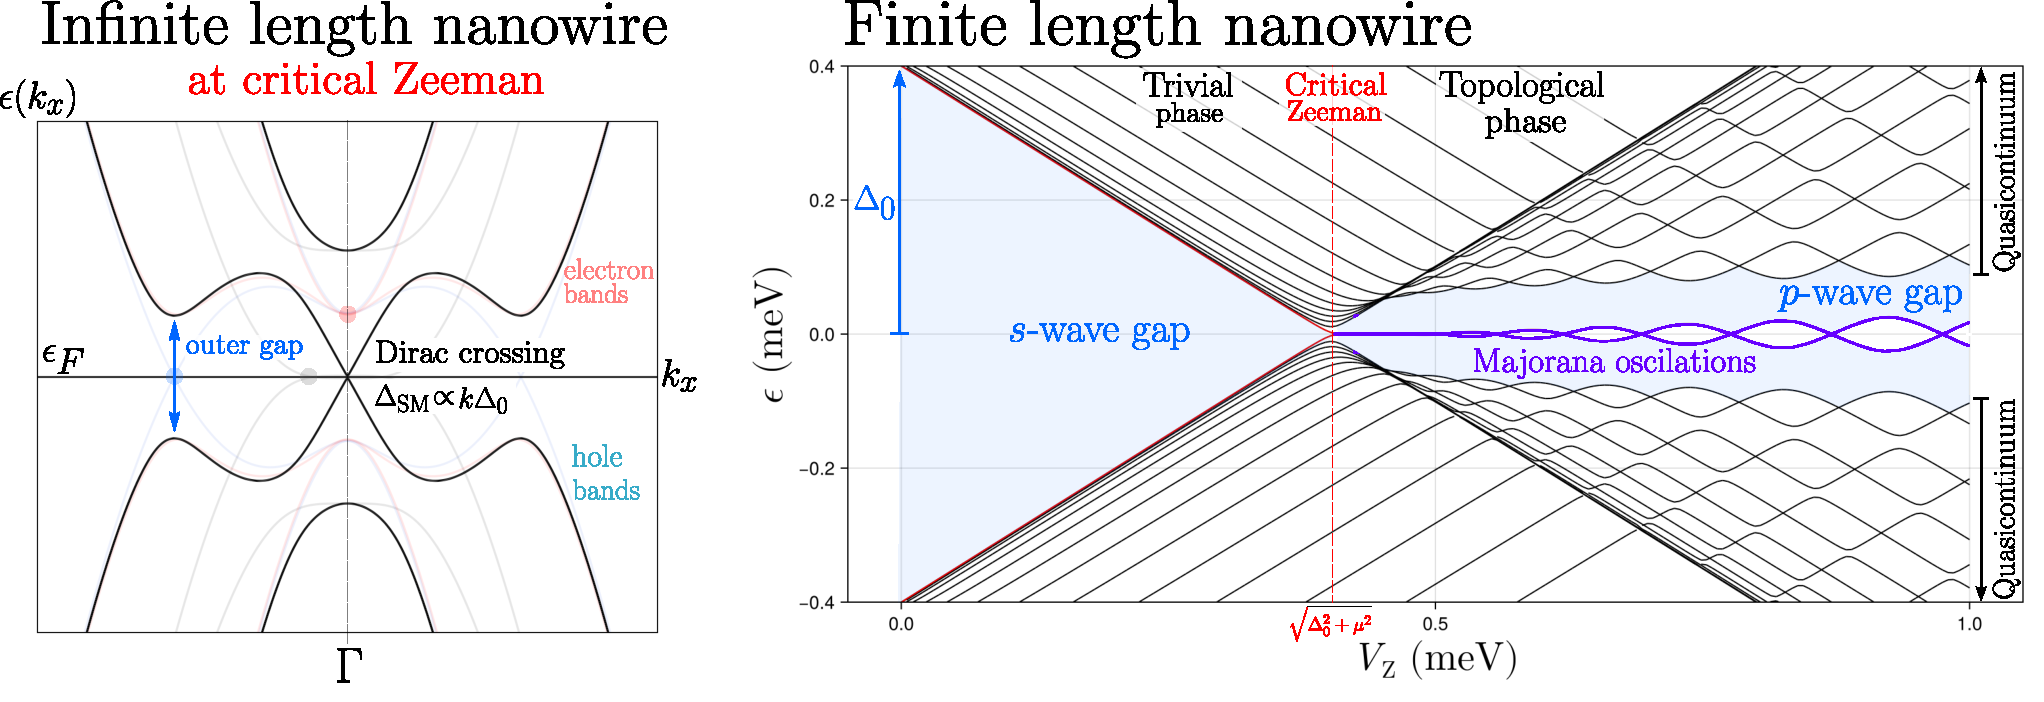
\includegraphics[scale=0.36]{images/lutchyn2}
\end{figure}
\end{center}

\end{frame}

%------------------------------------------------------------
{\usebackgroundtemplate{
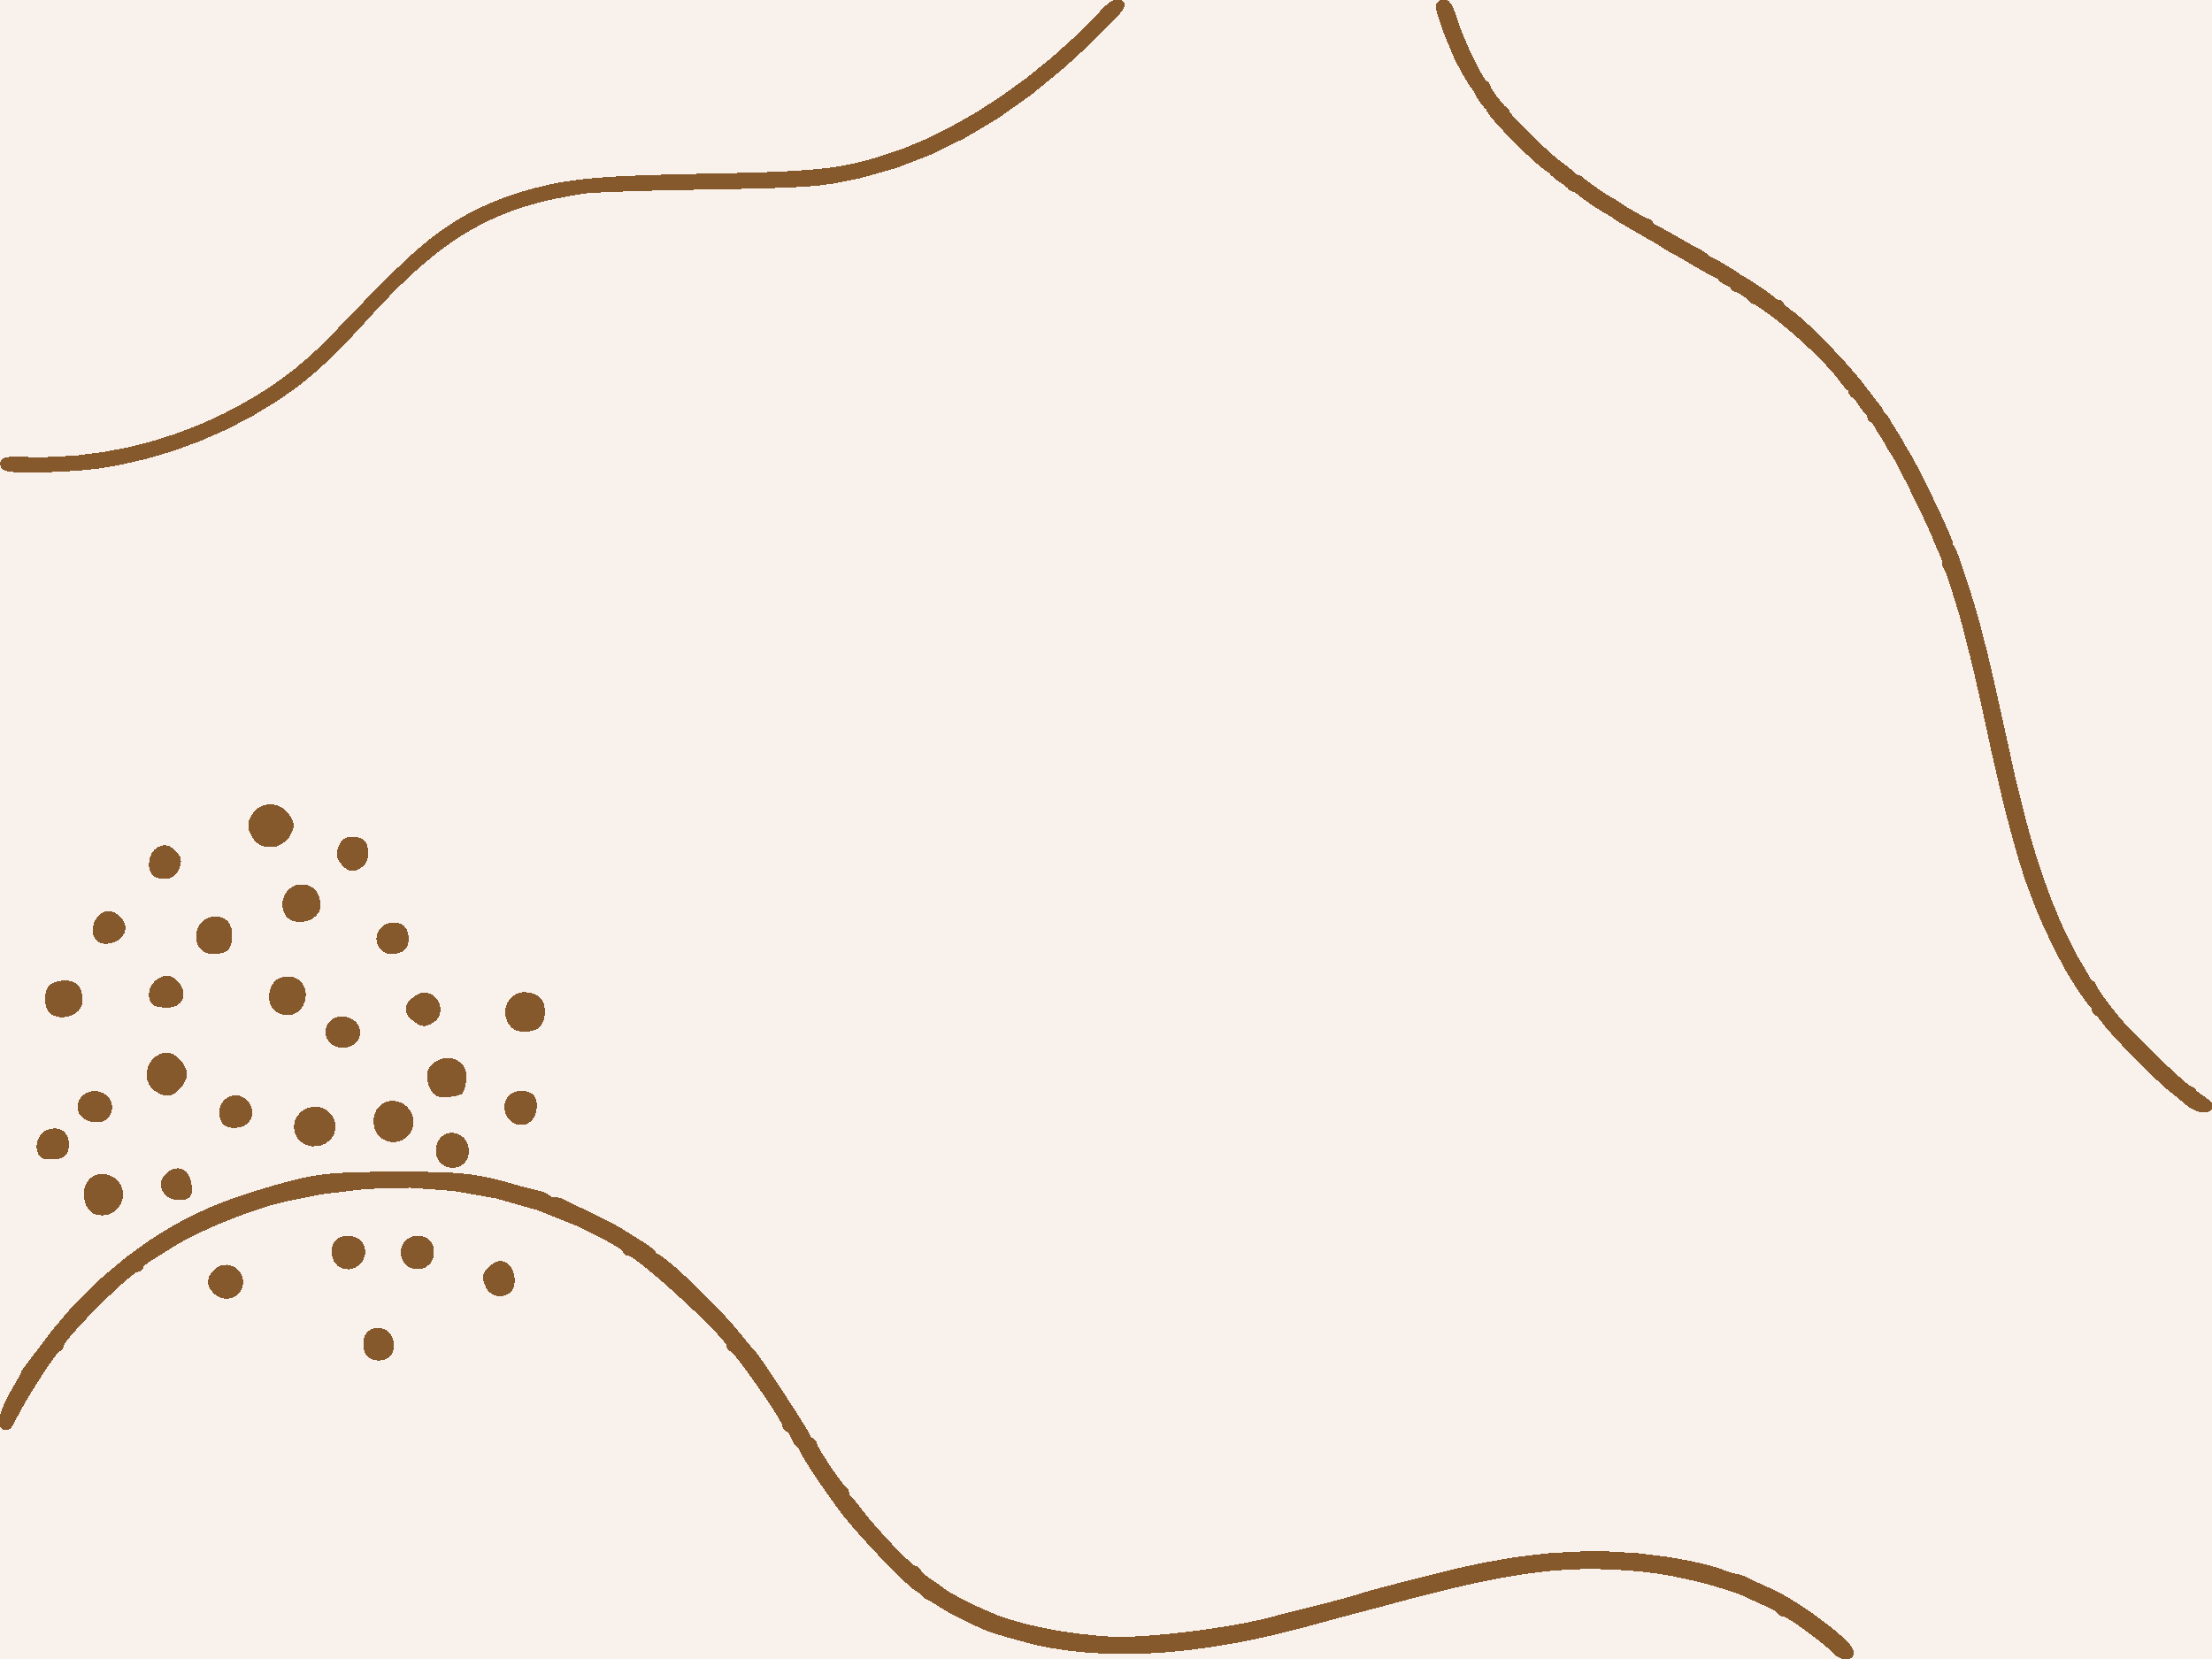
\includegraphics[width=\paperwidth,height=\paperheight]{images/assets/transition}}
\begin{frame}[noframenumbering]

\begin{center}
\Huge \textcolor{brown!70!black}{\textbf{Self-consistent}} \\
\Huge \textcolor{brown!70!black}{\textbf{HFB Majorana}} \\
\Huge \textcolor{brown!70!black}{\textbf{nanowires}}
\end{center}

\end{frame}}

%------------------------------------------------------------
\begin{frame}
\frametitle{Self-consistent HFB Majorana nanowires}

\vspace*{-5mm}
\begin{center}
\begin{figure}
\hspace*{-3mm}
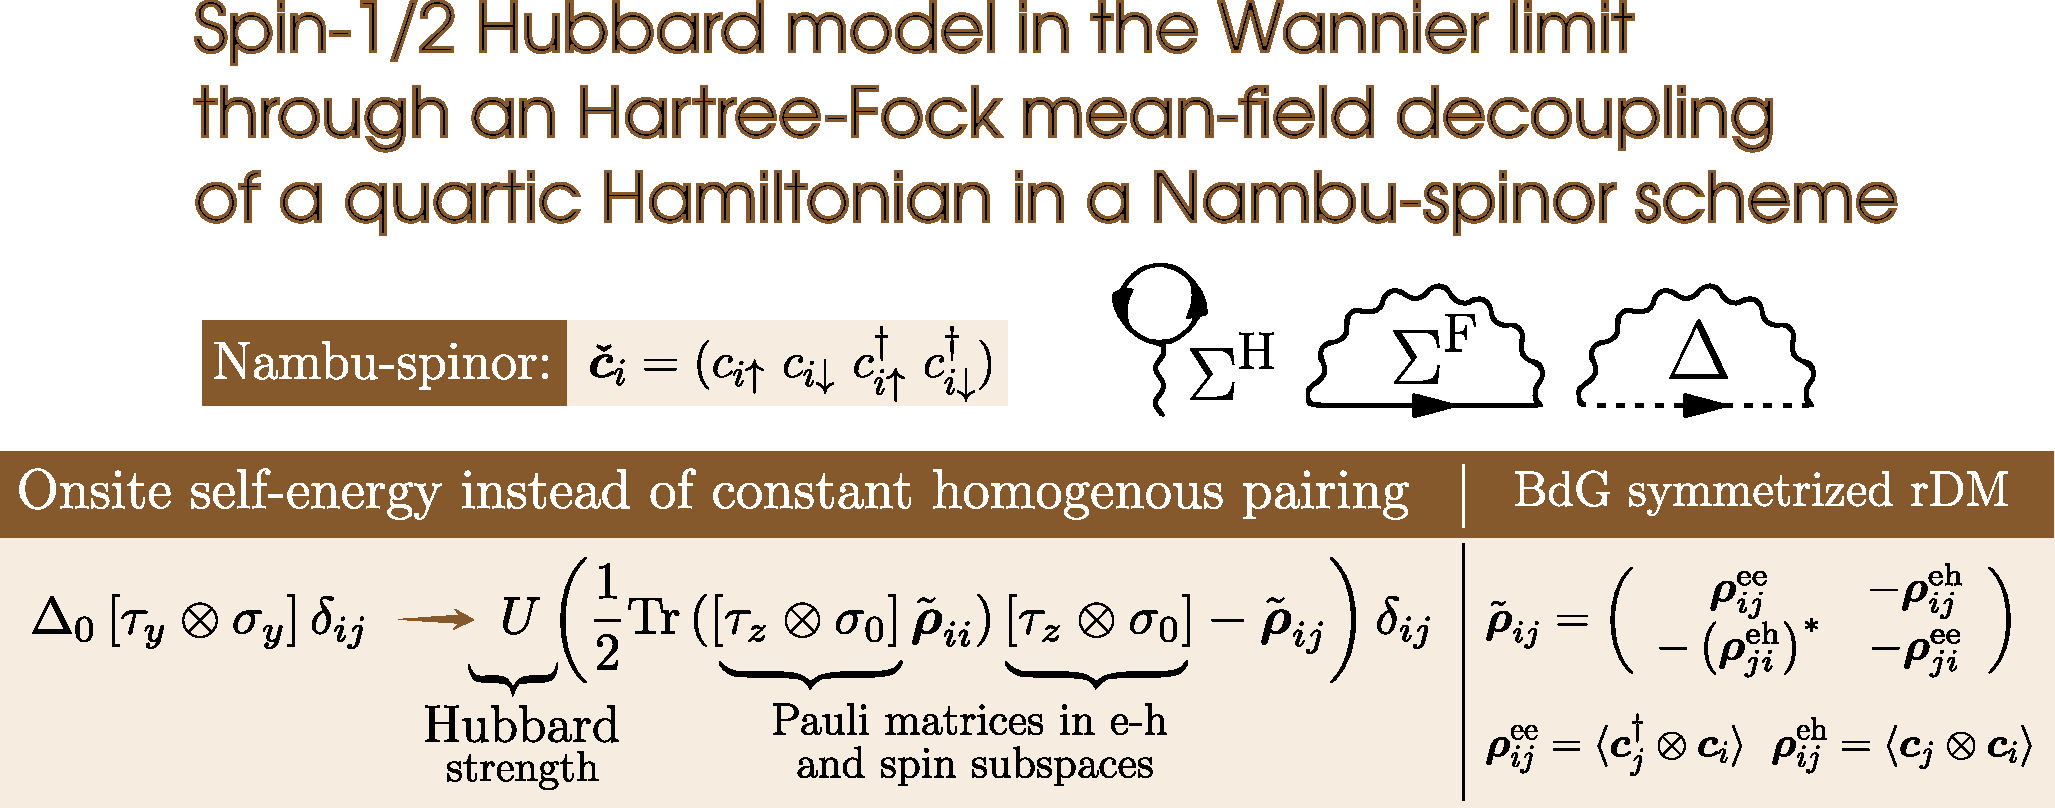
\includegraphics[scale=0.36]{images/theory}
\end{figure}
\end{center}

\pause
\begin{center}
\begin{figure}
\hspace*{-3mm}
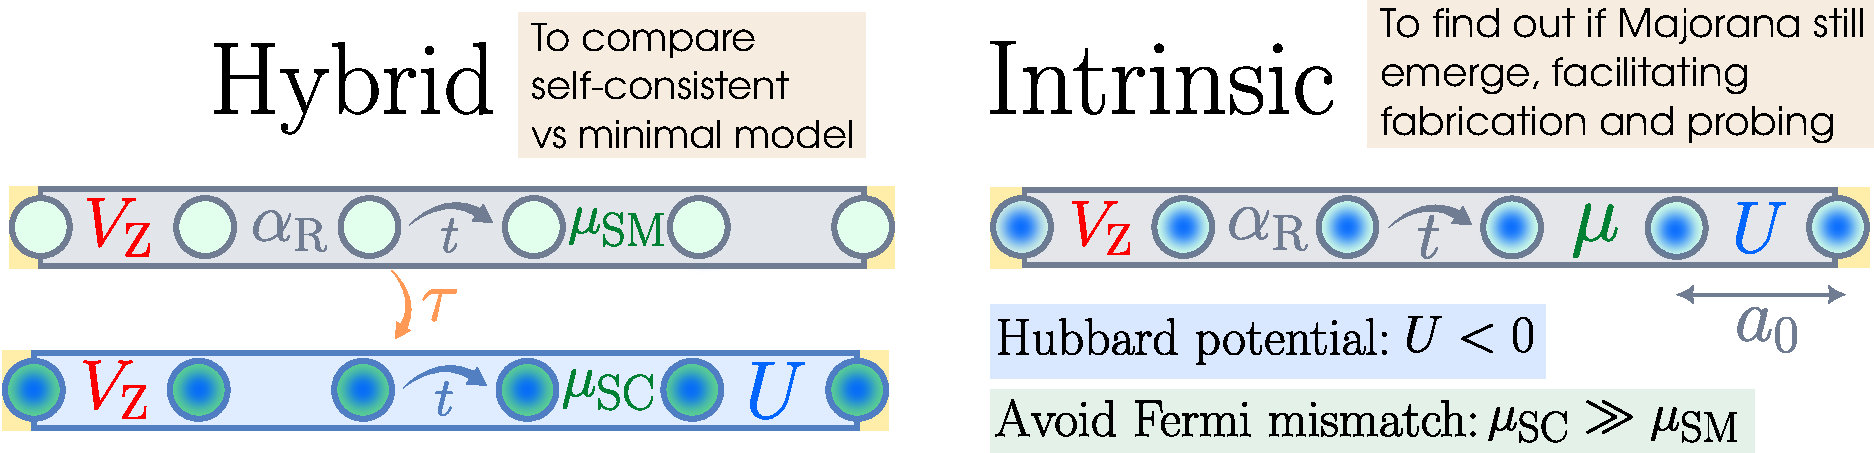
\includegraphics[scale=0.36]{images/models}
\end{figure}
\end{center}


\end{frame}

%------------------------------------------------------------
{\usebackgroundtemplate{
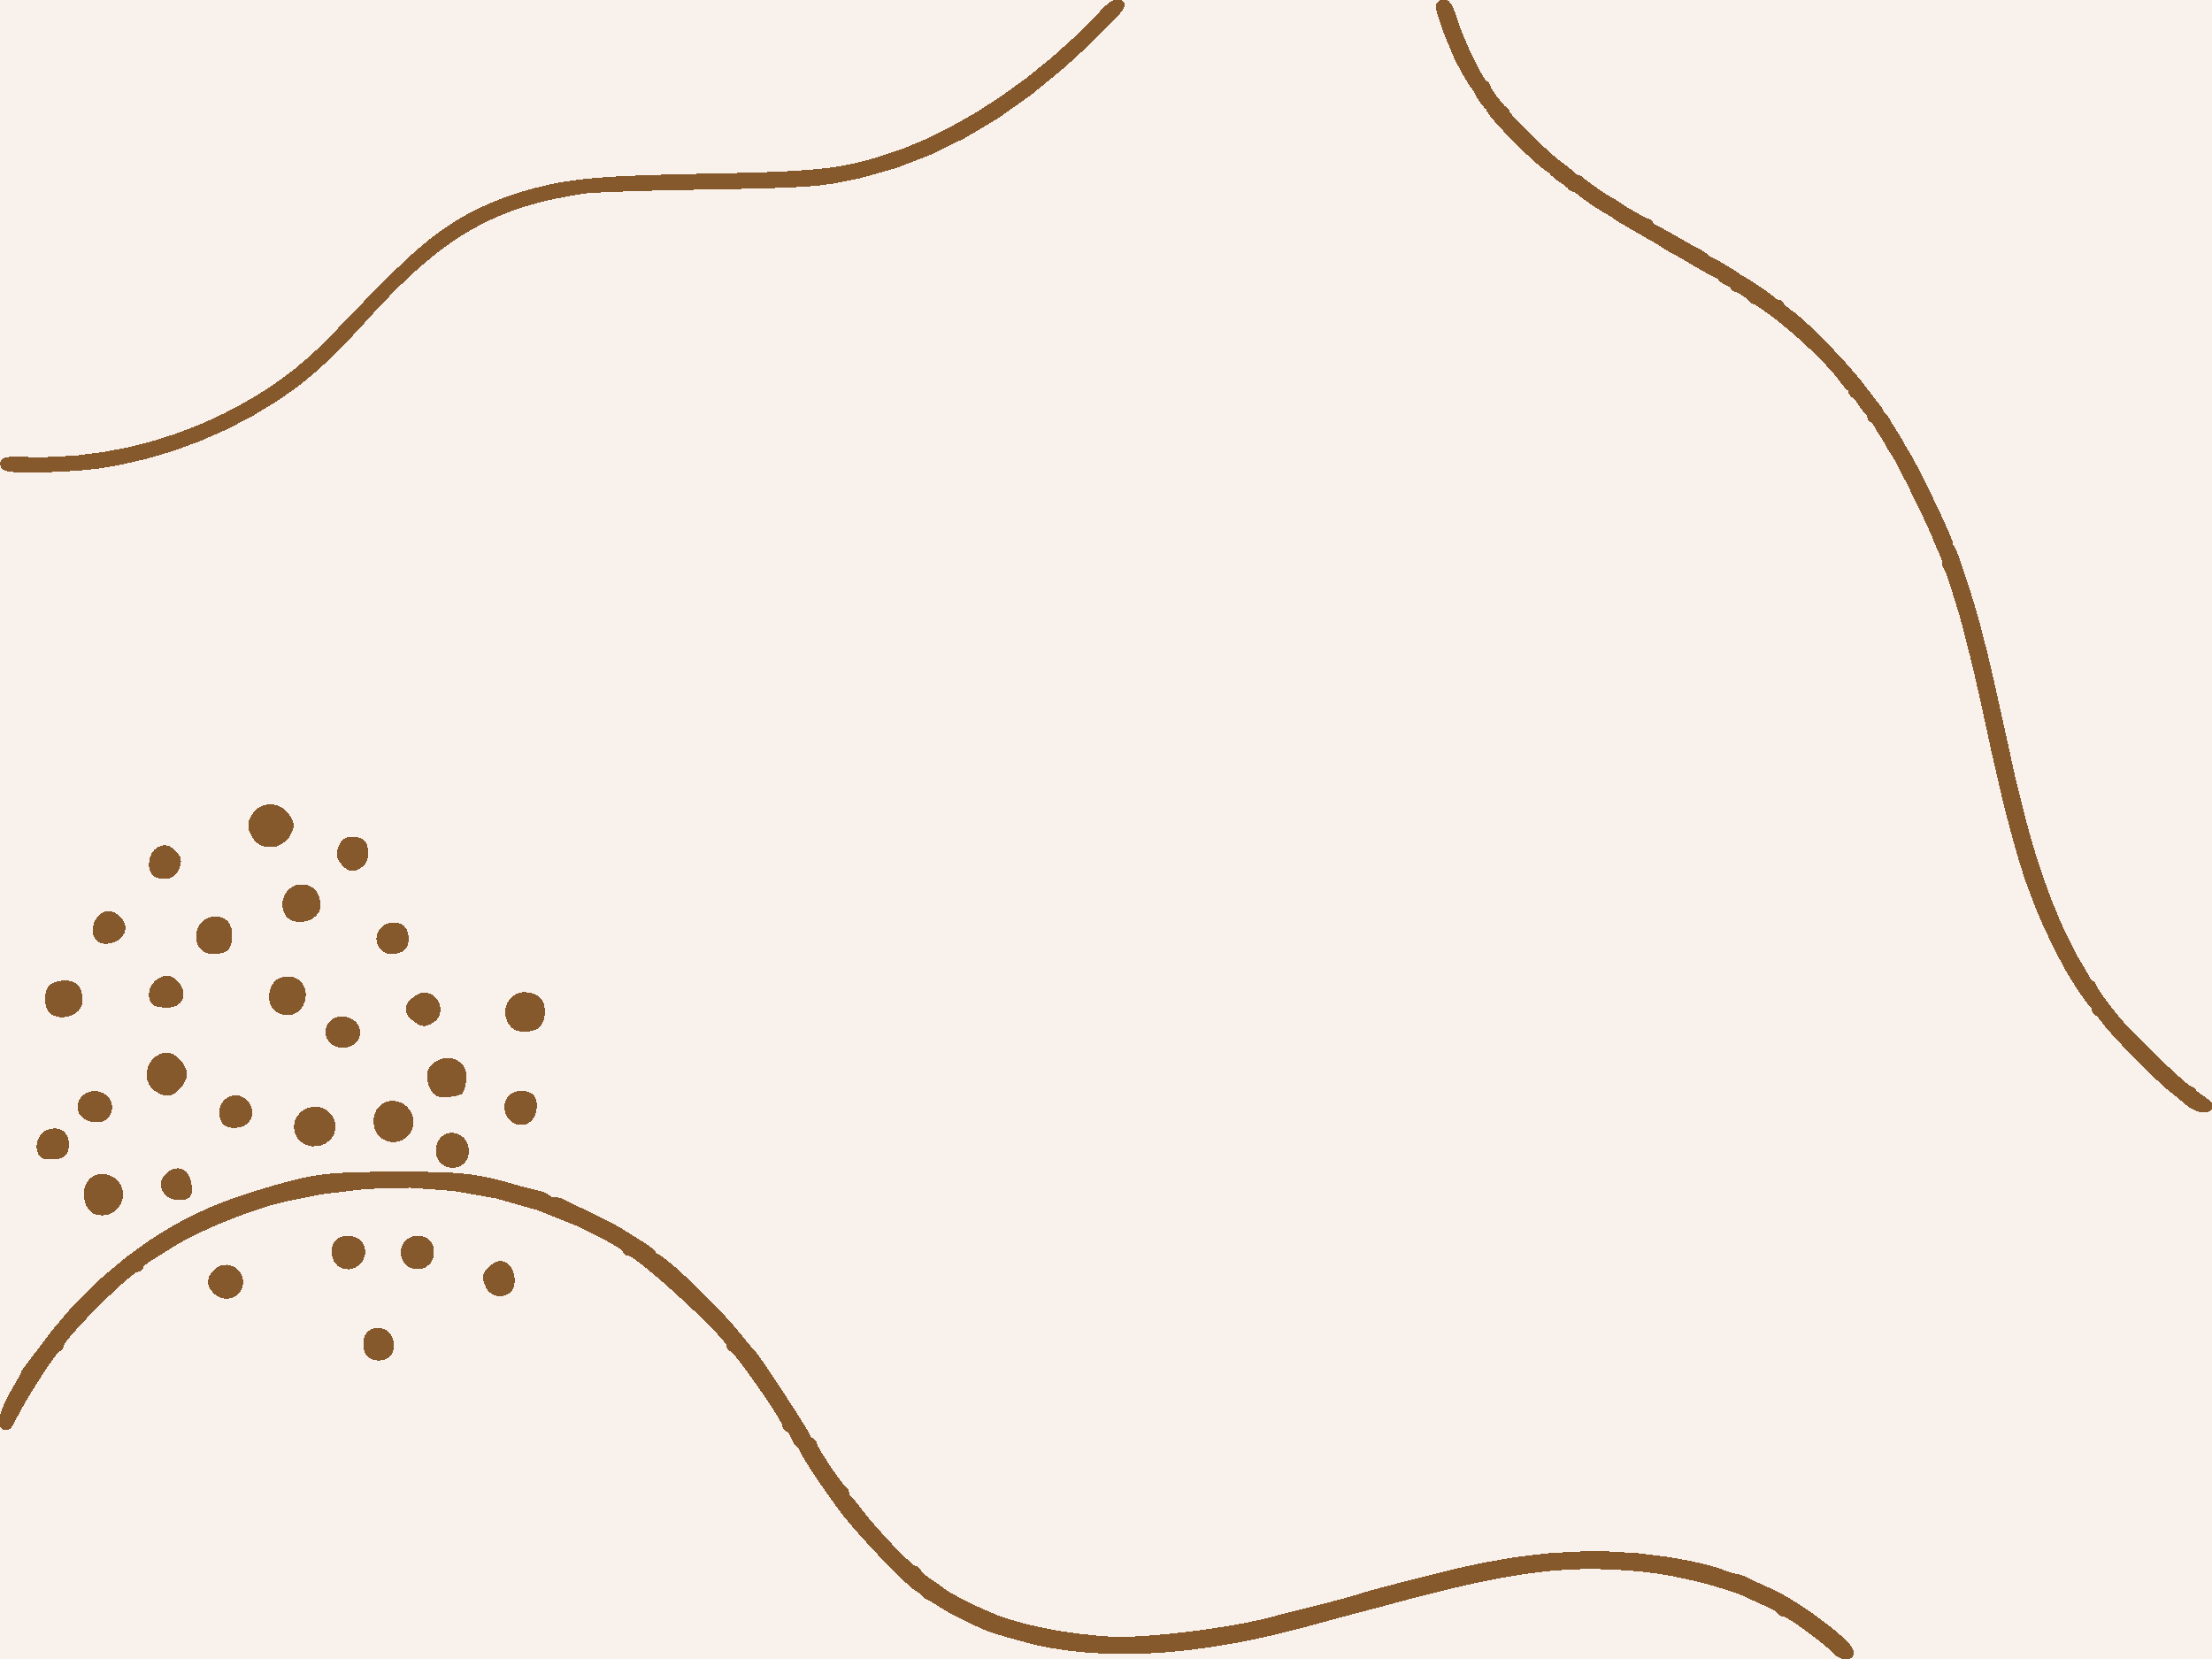
\includegraphics[width=\paperwidth,height=\paperheight]{images/assets/transition}}
\begin{frame}[noframenumbering]

\begin{center}
\Huge \textcolor{brown!70!black}{\textbf{Results}}
\end{center}

\end{frame}}

%------------------------------------------------------------
\begin{frame}
\frametitle{Self-consistent Majorana nanowires: \textcolor{black}{\underline{infinite hybrid wire}}}

\begin{center}
\begin{figure}

\includegraphics[scale=0.35]{images/hybrid_infinite}
\end{figure}
\end{center}


\end{frame}

%------------------------------------------------------------
\begin{frame}[noframenumbering]
\frametitle{Self-consistent Majorana nanowires: \textcolor{black}{\underline{infinite hybrid wire}}}

\begin{center}
\begin{figure}
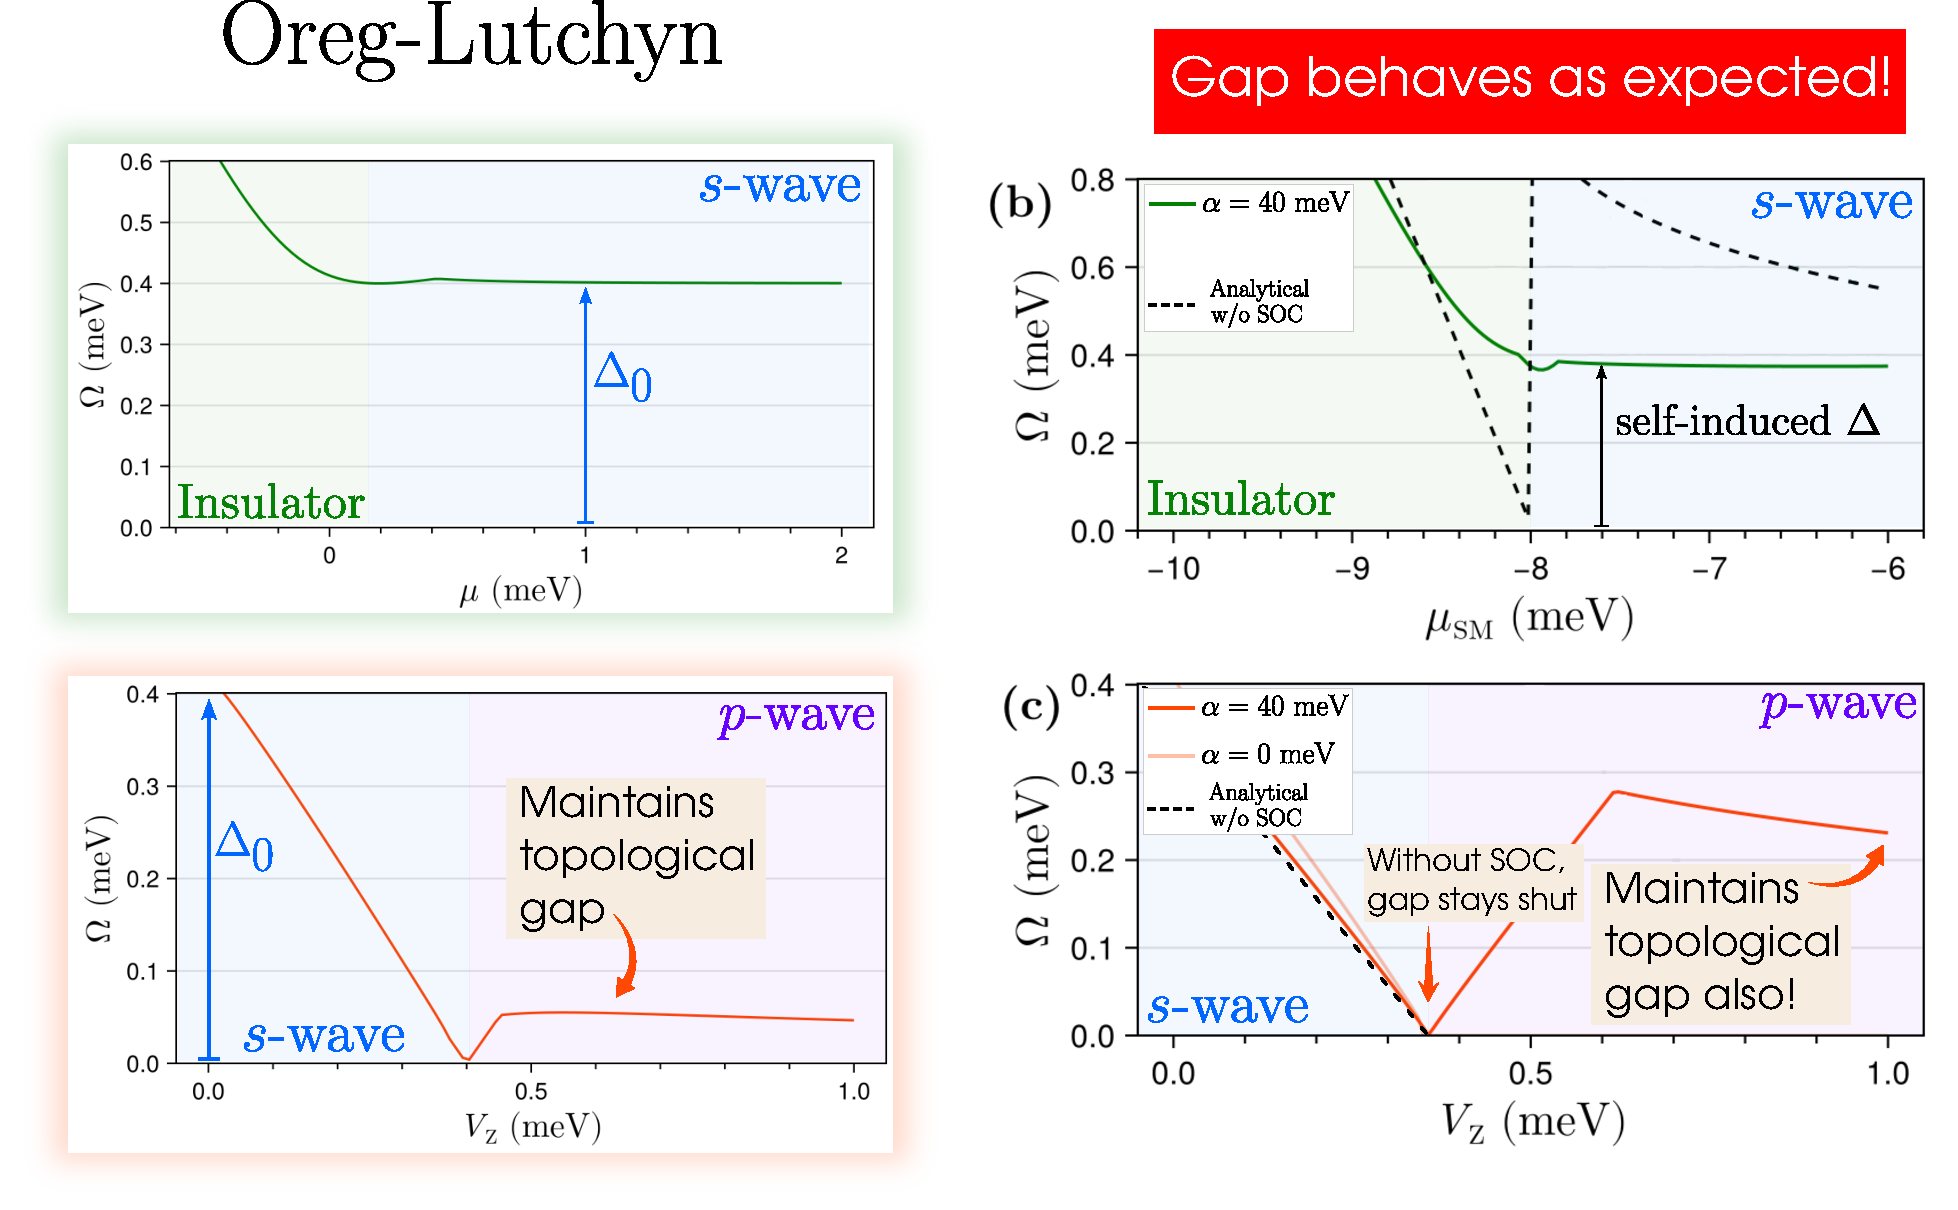
\includegraphics[scale=0.35]{images/hybrid_infinite_lutchyn}
\end{figure}
\end{center}

\end{frame}

%------------------------------------------------------------
\begin{frame}
\frametitle{Self-consistent Majorana nanowires: \textcolor{black}{\underline{finite hybrid wire}}}

\begin{center}
\begin{figure}

\includegraphics[scale=0.35]{images/hybrid_finite}
\end{figure}
\end{center}

\end{frame}

%------------------------------------------------------------
\begin{frame}
\frametitle{Self-consistent Majorana nanowires: \textcolor{black}{\underline{infinite intrinsic wire}}}

\begin{center}
\begin{figure}
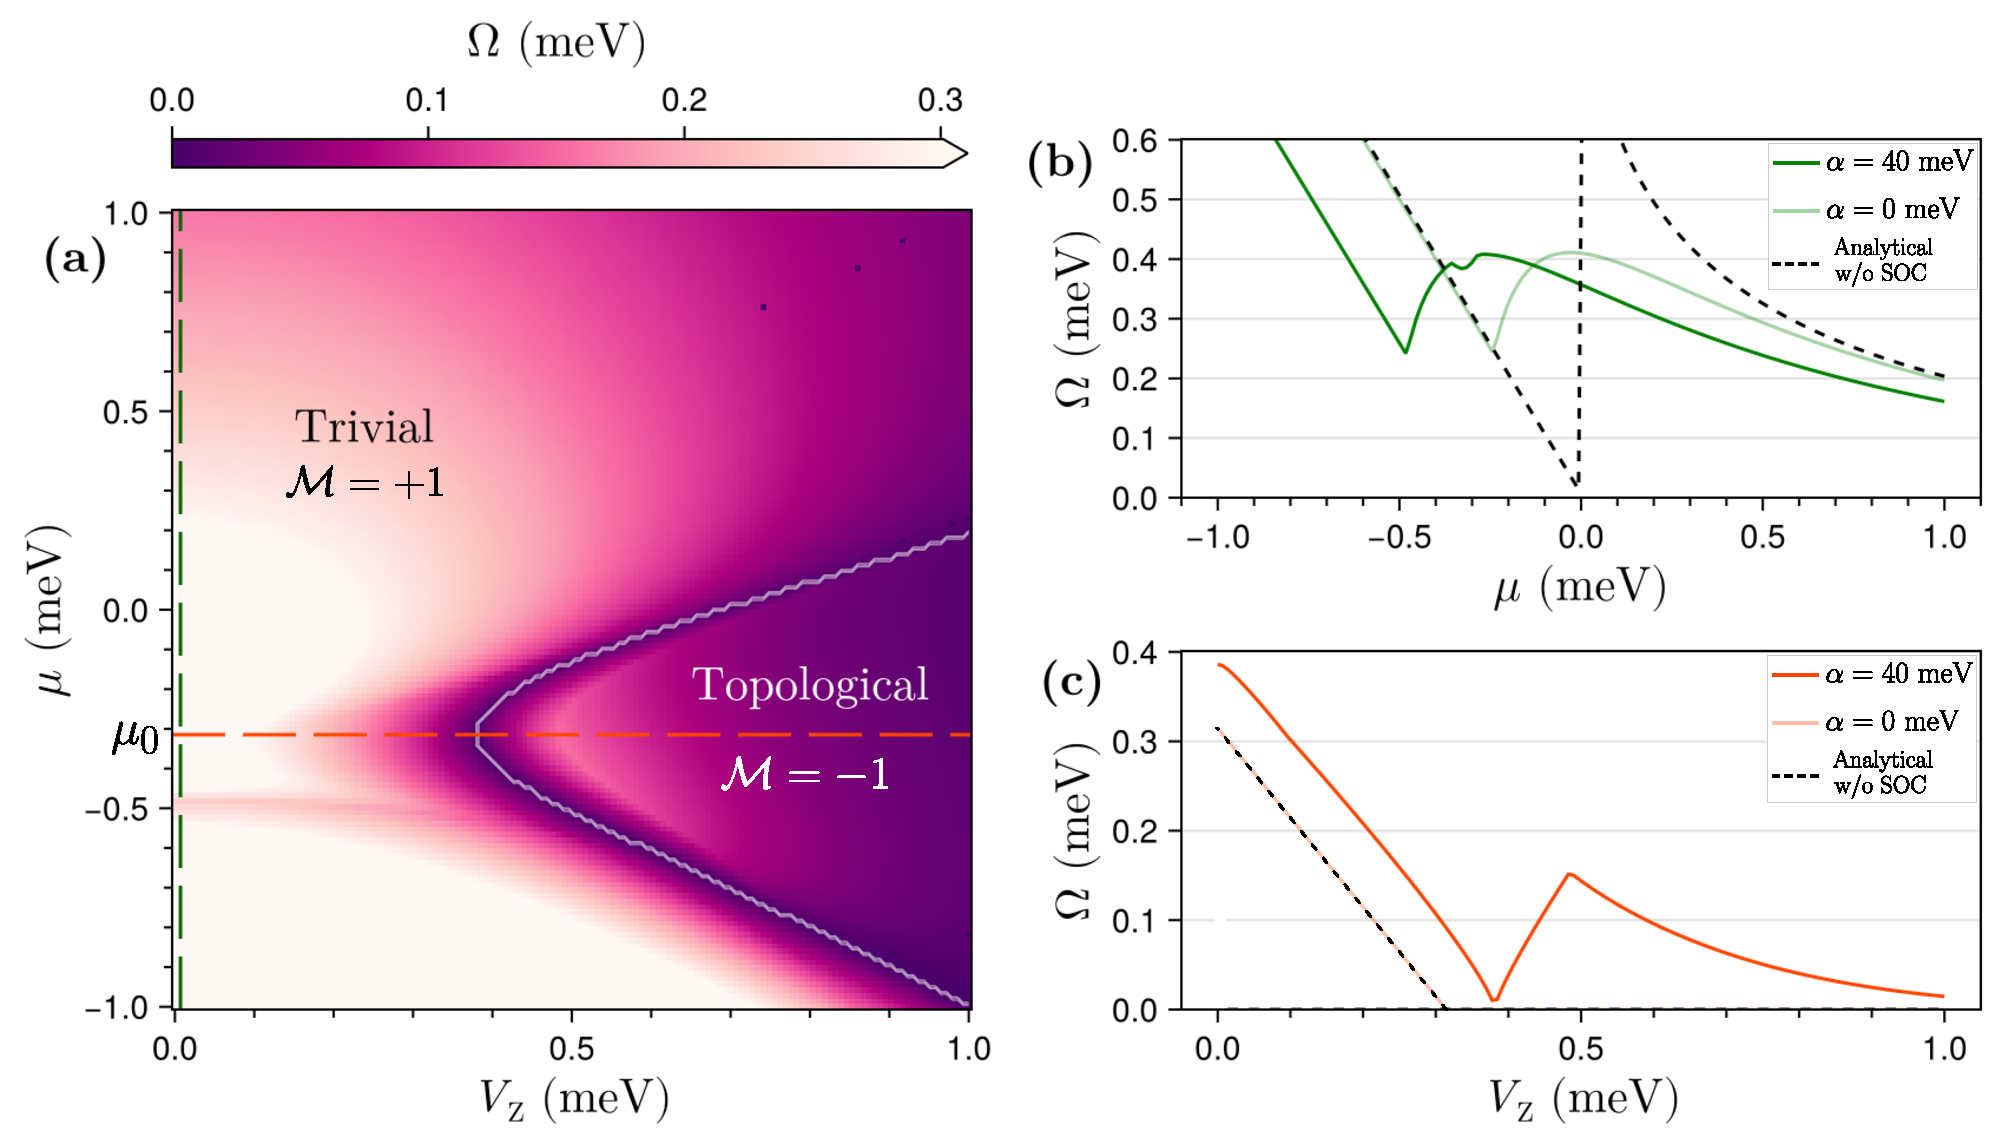
\includegraphics[scale=0.35]{images/intrinsic_infinite}
\end{figure}
\end{center}

\end{frame}

%------------------------------------------------------------
\begin{frame}[noframenumbering]
\frametitle{Self-consistent Majorana nanowires: \textcolor{black}{\underline{infinite intrinsic wire}}}

\begin{center}
\begin{figure}
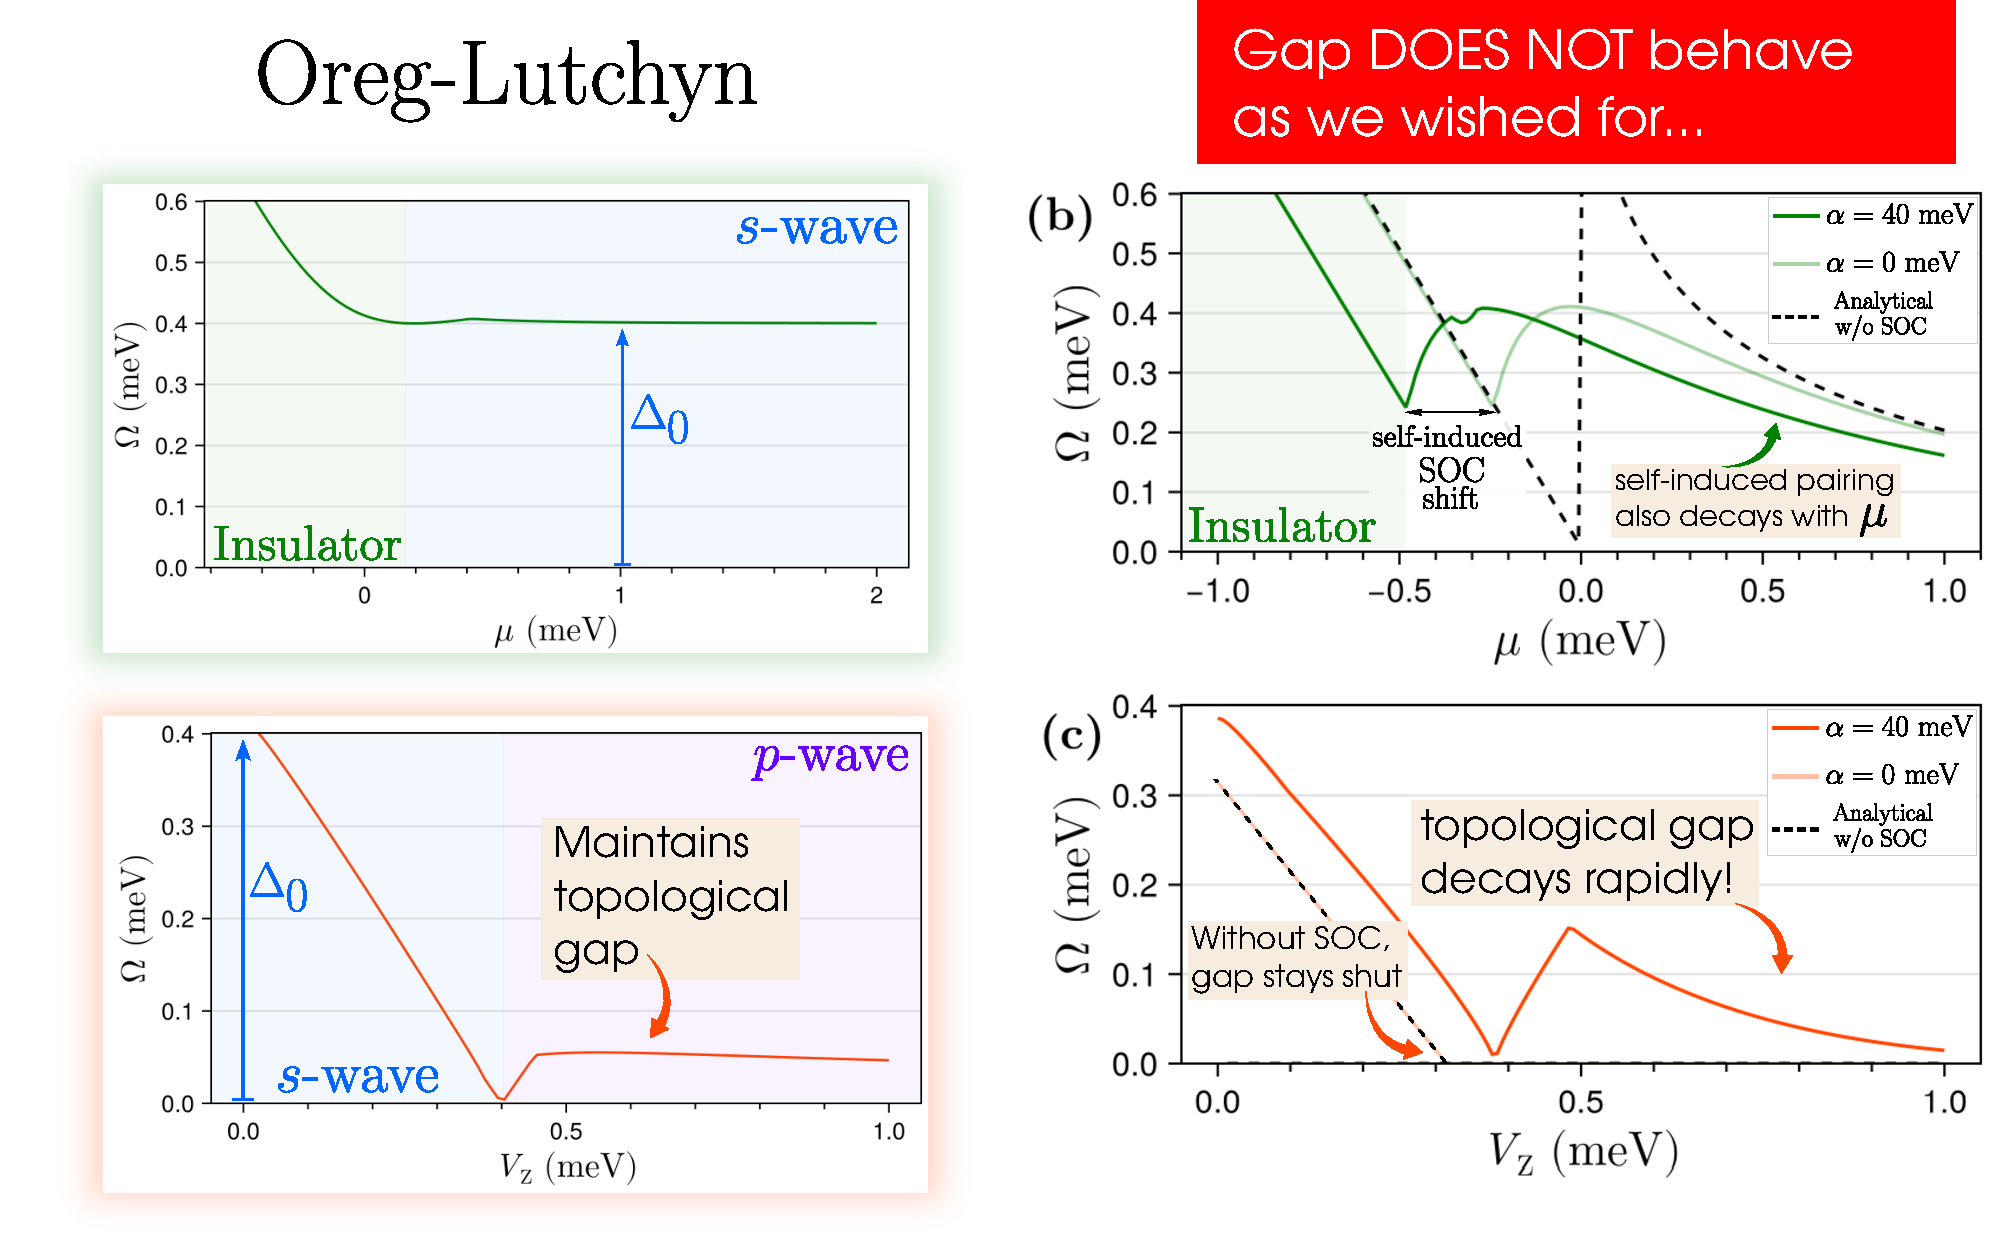
\includegraphics[scale=0.35]{images/intrinsic_infinite_lutchyn}
\end{figure}
\end{center}

\end{frame}

%------------------------------------------------------------
\begin{frame}
\frametitle{Self-consistent Majorana nanowires: \textcolor{black}{\underline{finite intrinsic wire}}}

\begin{center}
\begin{figure}
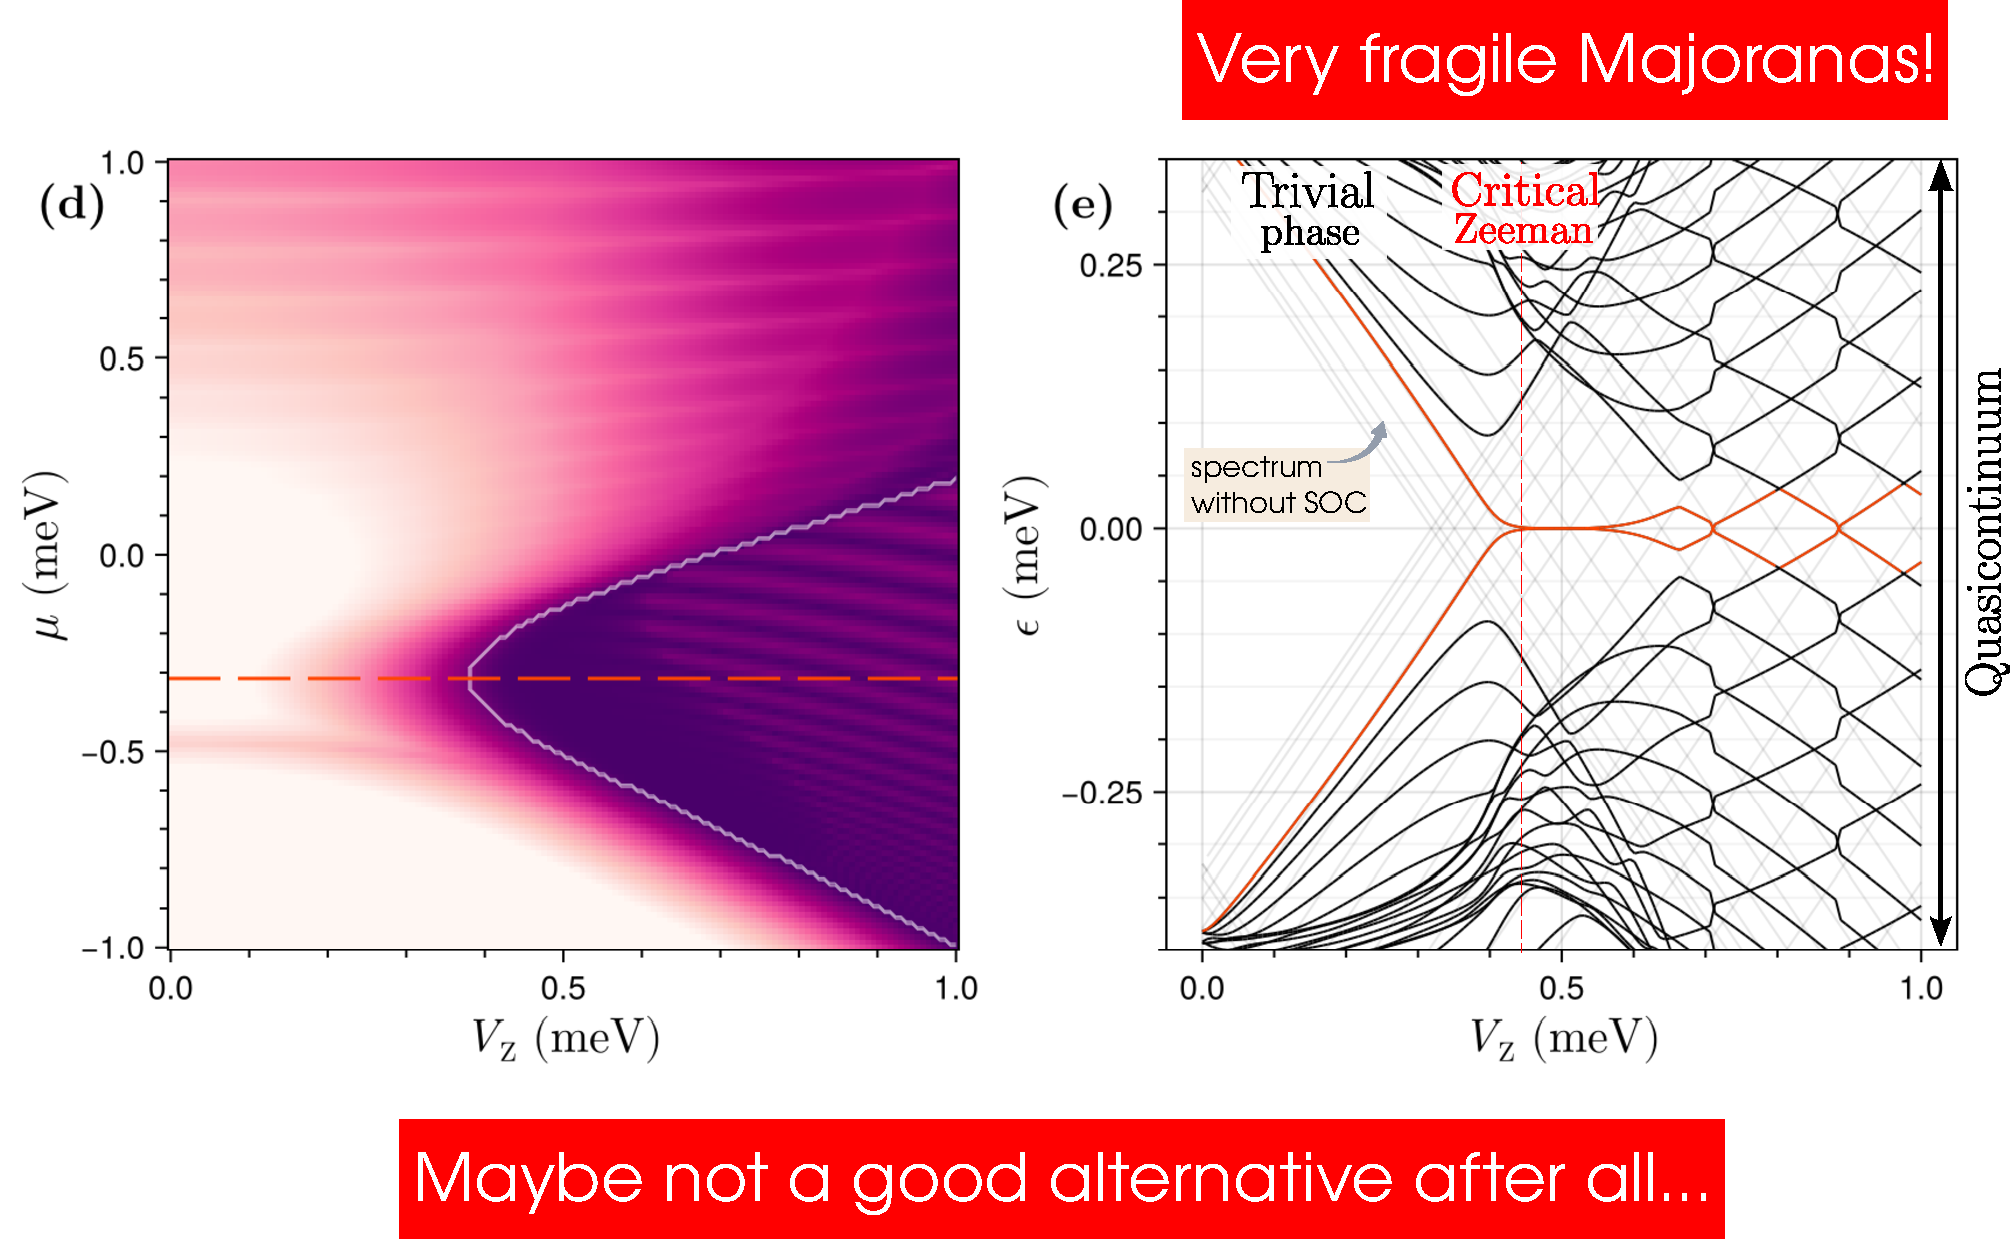
\includegraphics[scale=0.35]{images/intrinsic_finite}
\end{figure}
\end{center}

\end{frame}

%------------------------------------------------------------
{\usebackgroundtemplate{

\includegraphics[width=\paperwidth,height=\paperheight]{images/assets/transition3}}
\begin{frame}[noframenumbering]

\vspace*{-40mm}
\begin{center}
\Huge \textcolor{brown!70!black}{\textbf{Thank you for listening!}} \\
\Huge \textcolor{brown!70!black}{\textbf{Any questions?}}
\end{center}

\end{frame}}

%------------------------------------------------------------
{\usebackgroundtemplate{
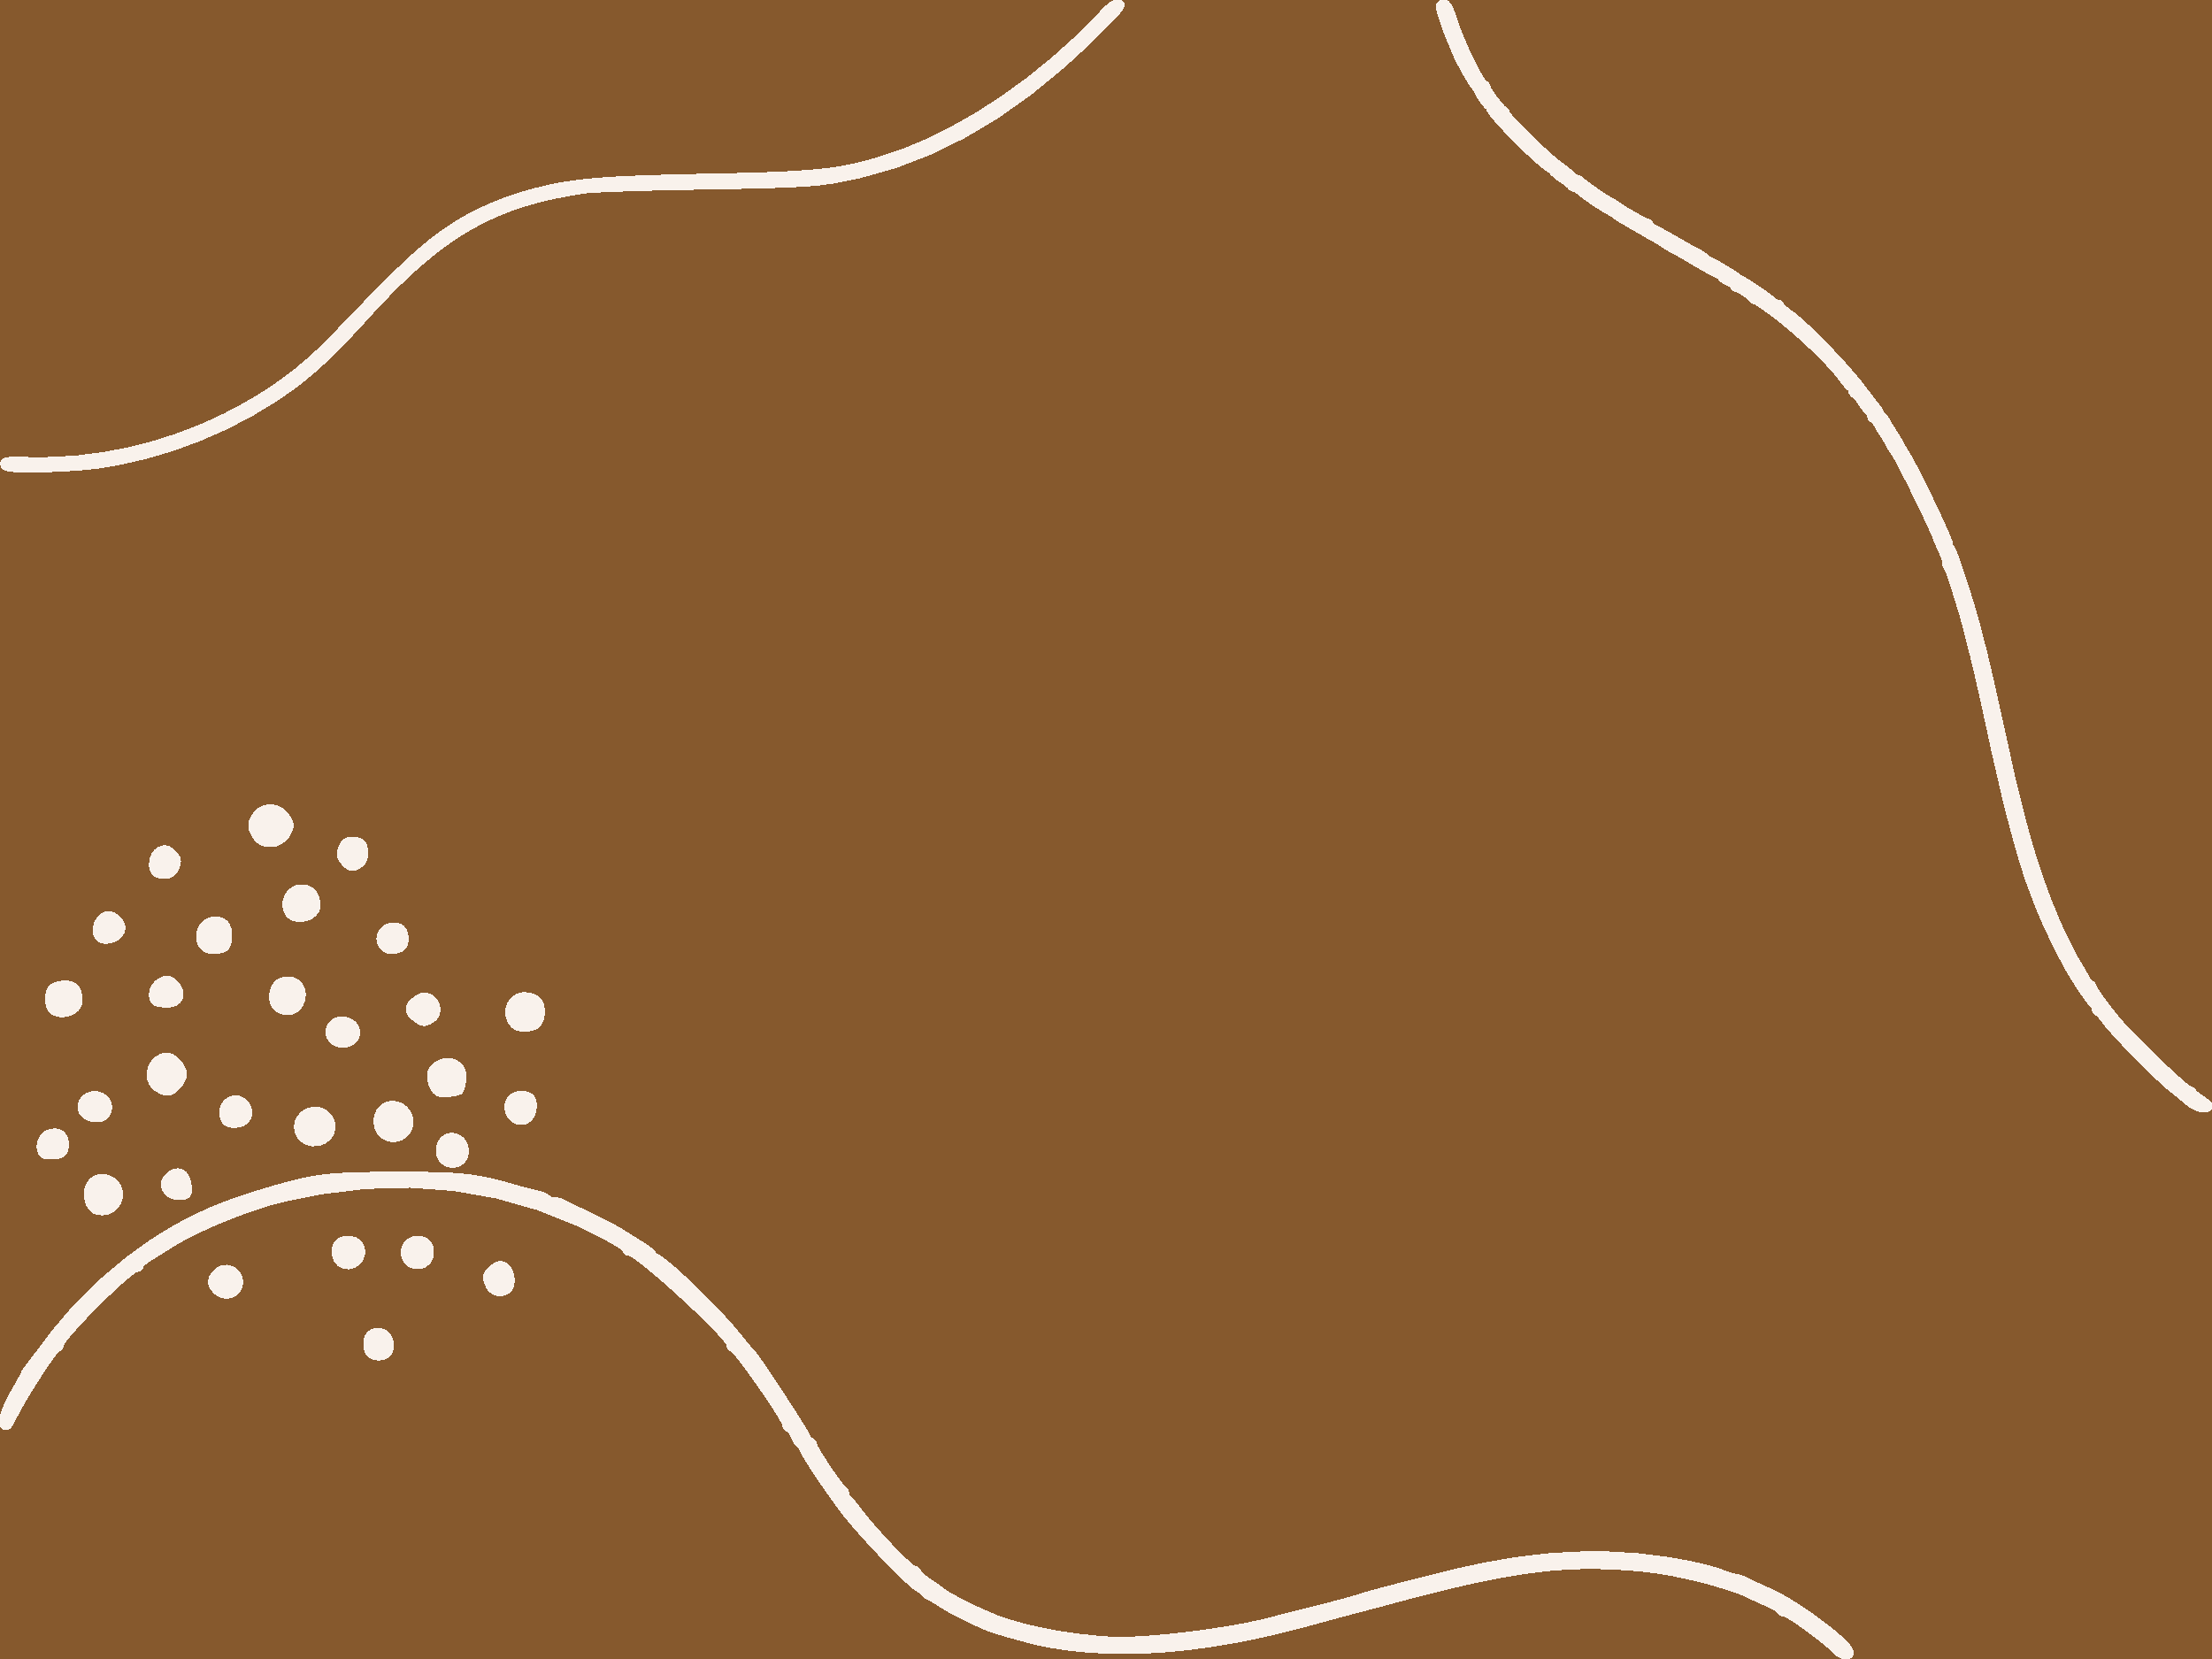
\includegraphics[width=\paperwidth,height=\paperheight]{images/assets/transition2}}
\begin{frame}[noframenumbering]

\begin{center}
\Huge \textcolor{brown!10!white}{\textbf{Appendix}}
\end{center}

\end{frame}}

%------------------------------------------------------------
{\usebackgroundtemplate{
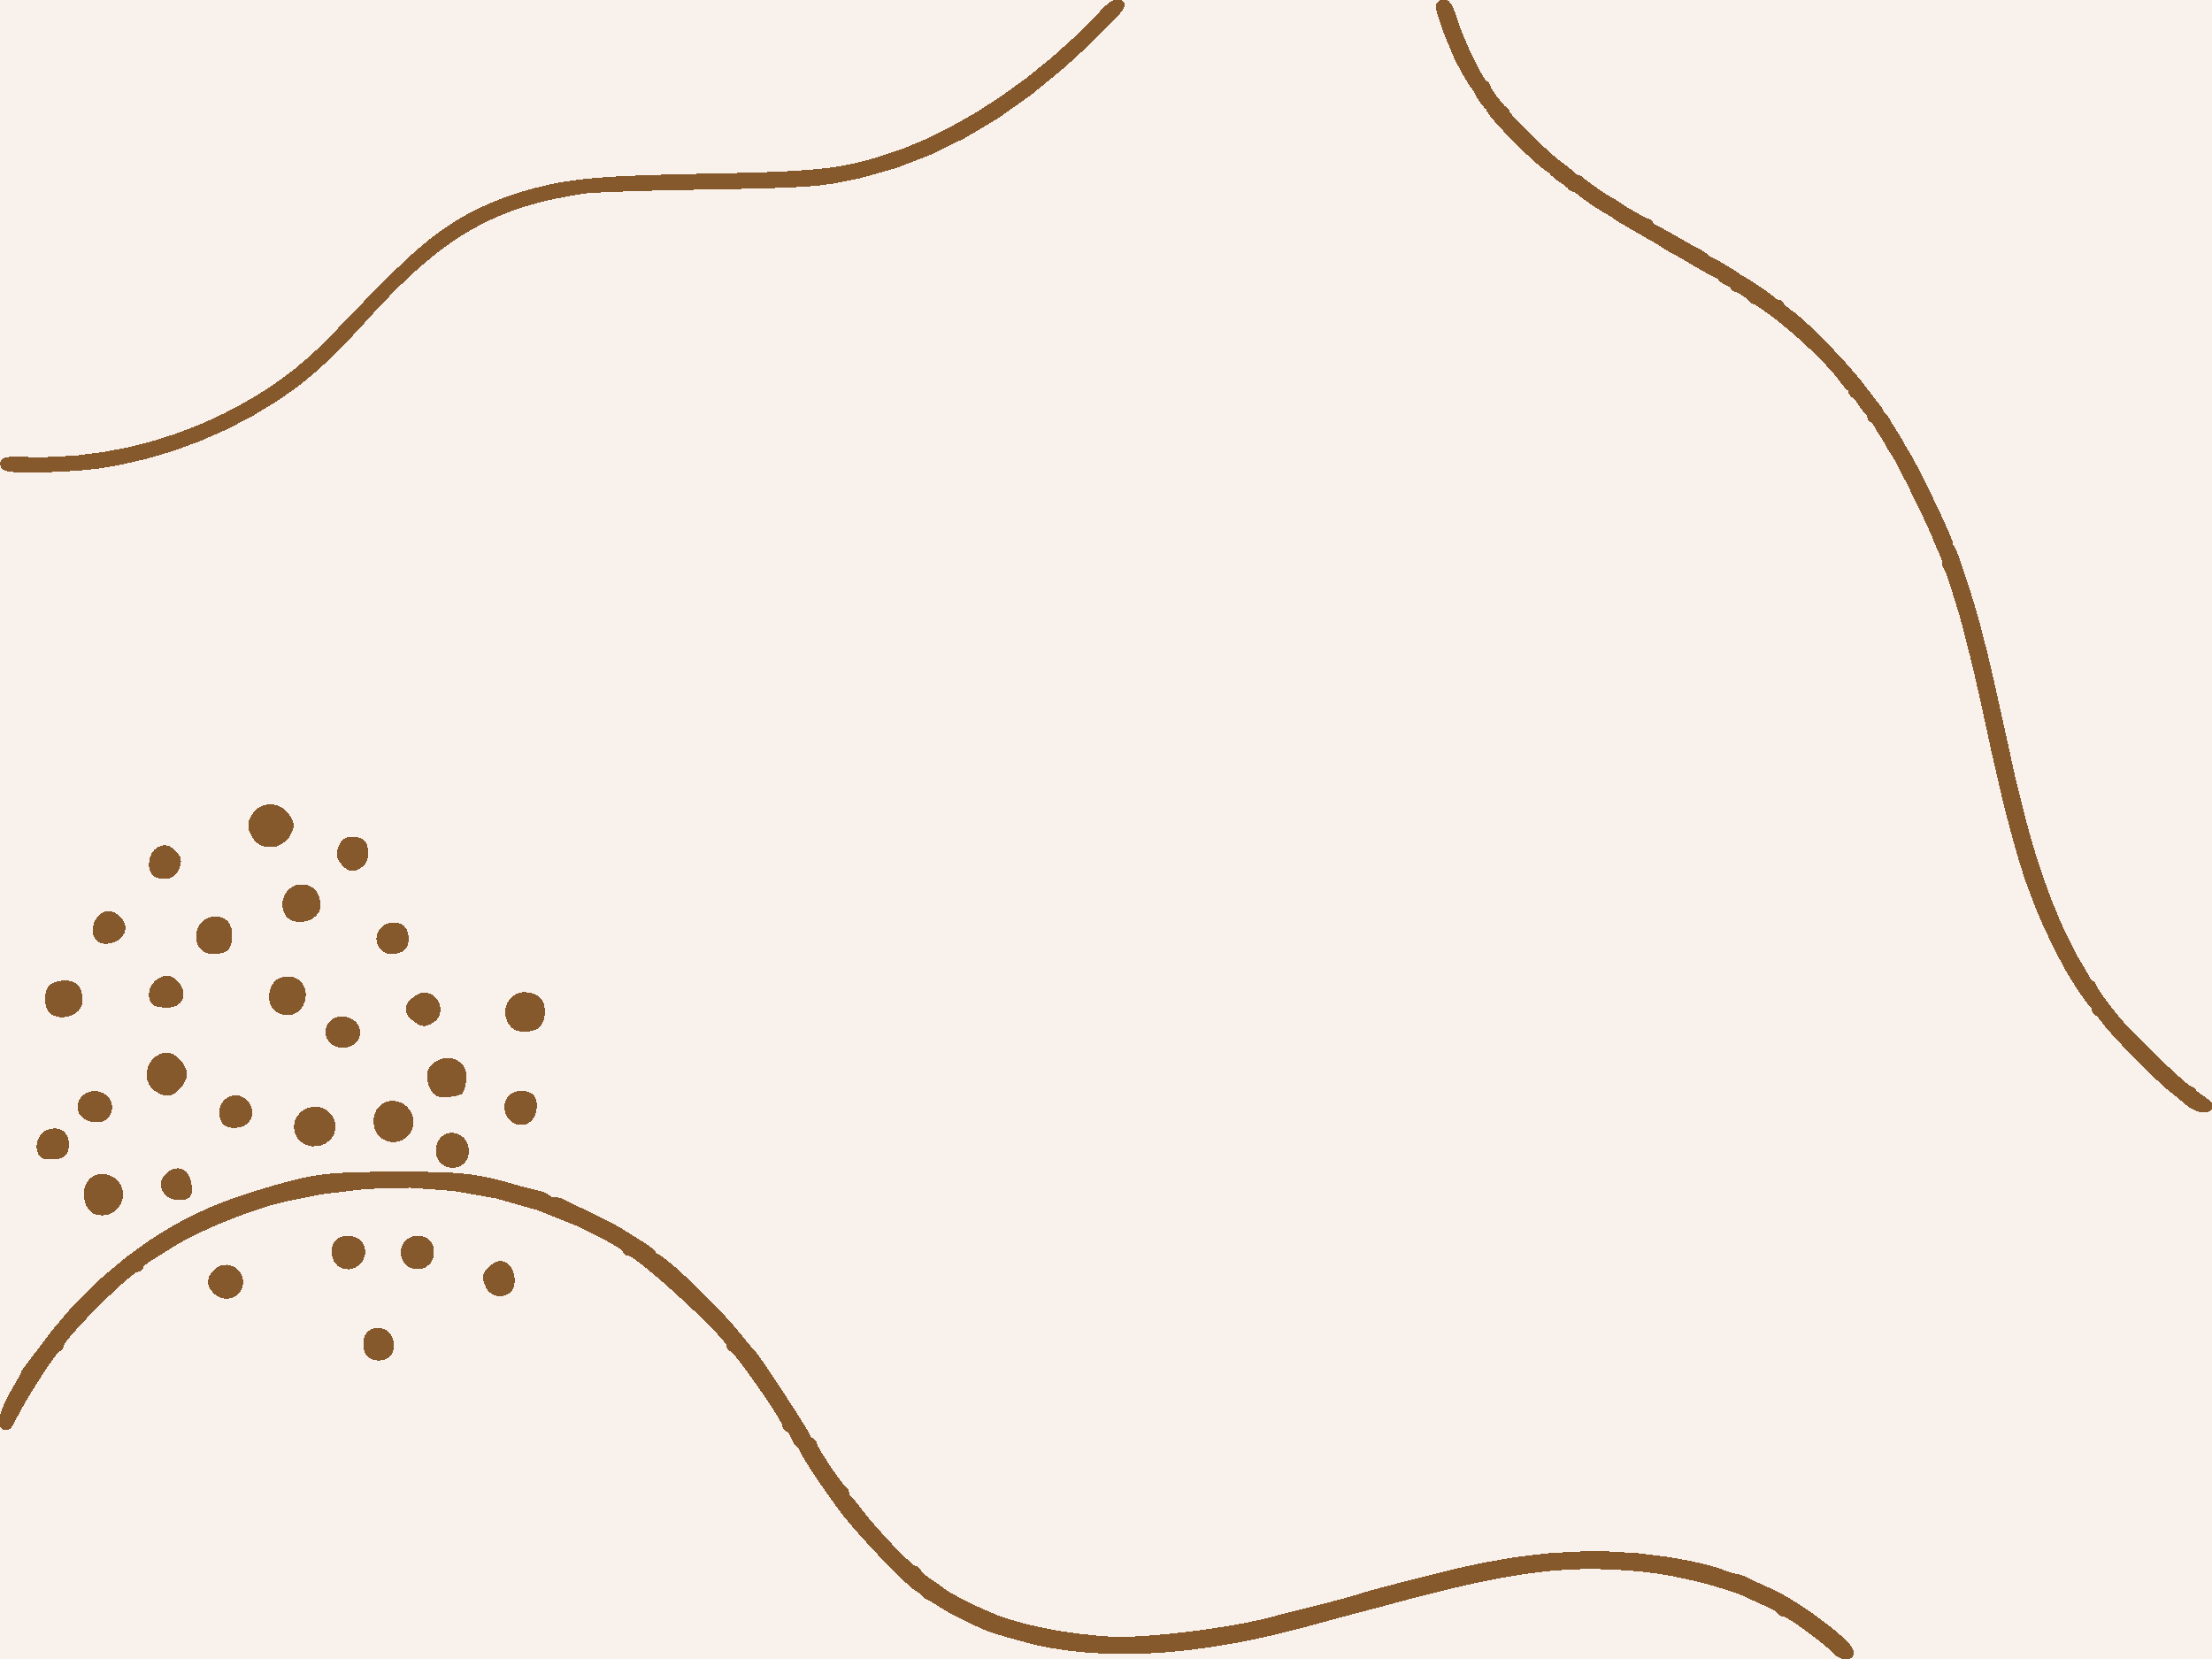
\includegraphics[width=\paperwidth,height=\paperheight]{images/assets/transition}}
\begin{frame}[noframenumbering]

\begin{center}
\Huge \textcolor{brown!70!black}{\textbf{Hartree-Fock-Bogoliubov}} \\
\Huge \textcolor{brown!70!black}{\textbf{mean-field theory}}
\end{center}

\end{frame}}

%------------------------------------------------------------
\begin{frame}[noframenumbering]
\frametitle{Hartree-Fock-Bogoliubov mean-field theory}

\begin{exampleblock}{Many-body system of electrons}
\begin{equation*}
\hat{H}=\sum_{\alpha\beta}h_{\alpha\beta}c_{\alpha}^{\dagger}c_{\beta}+\frac{1}{2}\sum_{\alpha\beta\gamma\delta}V_{\gamma\delta}^{\alpha\beta}c_{\alpha}^{\dagger}c_{\beta}^{\dagger}c_{\gamma}c_{\delta}
\end{equation*}
\end{exampleblock}
\pause

\begin{columns}
\column{2.5cm}
\begin{alertblock}{Nambu spinor}
\vspace*{-4.5mm}
\begin{equation*}
\check{c}_{a}=\left(\begin{array}{c}
c_{a}\\
c_{a}^{\dagger}
\end{array}\right)
\end{equation*}
\end{alertblock}
\pause

\column{7.5cm}
\begin{exampleblock}{Reduced density matrix (rDM)}
\vspace*{-4.5mm}
\begin{equation*}
\rho_{ab}=\left(\begin{array}{cc}
\langle c_{b}^{\dagger}c_{a}\rangle & \langle c_{b}c_{a}\rangle\\
\langle c_{b}^{\dagger}c_{a}^{\dagger}\rangle & \langle c_{b}c_{a}^{\dagger}\rangle
\end{array}\right)=\left(\begin{array}{cc}
\rho_{ab}^{\text{ee}} & \rho_{ab}^{\text{eh}}\\
\rho_{ab}^{\text{he}} & \rho_{ab}^{\text{hh}}
\end{array}\right)
\end{equation*}
\end{exampleblock}
\pause
\end{columns}

\vspace*{4,5mm}
\begin{itemize} 
\item Solve for the Heinsenberg equation of motion...
\end{itemize}
\pause

\begin{alertblock}{Mean-field decoupling}
\begin{equation*}
\langle c_{\alpha}^{\dagger}c_{\beta}^{\dagger}c_{\gamma}c_{\delta}\rangle\approx\mathfrak{\rho}_{\beta\alpha}^{\text{he}}\mathfrak{\rho}_{\delta\gamma}^{\text{eh}}-\rho_{\gamma\alpha}^{\text{ee}}\rho_{\delta\beta}^{\text{ee}}+\rho_{\delta\alpha}^{\text{ee}}\rho_{\gamma\beta}^{\text{ee}}
\end{equation*}
\end{alertblock}

\end{frame}

%------------------------------------------------------------
\begin{frame}[noframenumbering]
\frametitle{Hartree-Fock-Bogoliubov mean-field theory}

\begin{exampleblock}{rDM Bogoliubov-de Gennes EoM}
\begin{equation*}
i\hbar\frac{d}{dt}\rho_{ab}=\left[H_{ab}^{\text{BdG}},\rho_{ab}\right]\quad\text{with}\quad H_{\text{BdG}}=\left(\begin{array}{cc}
h_{ab}^{\text{HF}} & \Delta_{ab}\\
\Delta_{ba}^{*} & -h_{ba}^{\text{HF}}
\end{array}\right)
\end{equation*}
\end{exampleblock}
\pause

\begin{columns}
\column{2.5cm}
\begin{center}
\begin{figure}
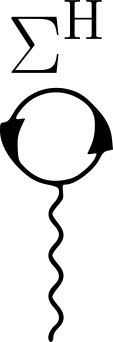
\includegraphics[scale=0.5]{images/H}
\end{figure}
\end{center}

\column{4.5cm}
\begin{alertblock}{\centering{Hartree, Fock and \\pairing self-energies}}
\begin{align*}
\Sigma_{ab}^{H}=&\sum_{\gamma\delta}V_{b\gamma}^{\delta a}\rho_{\gamma\delta}^{\text{ee}}\\\Sigma_{ab}^{F}=&-\sum_{\gamma\delta}V_{b\gamma}^{a\delta}\rho_{\gamma\delta}^{\text{ee}}\\\Delta_{ab}=&\sum_{\gamma\delta}V_{\delta\gamma}^{ab}\rho_{\gamma\delta}^{\text{eh}}
\end{align*}
\end{alertblock}

\column{4cm}
\begin{center}
\begin{figure}
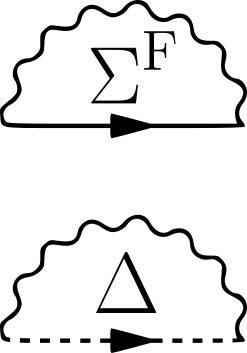
\includegraphics[scale=0.5]{images/FD}
\end{figure}
\end{center}
\end{columns}

\end{frame}

%------------------------------------------------------------
\begin{frame}[noframenumbering]
\frametitle{Hartree-Fock-Bogoliubov mean-field theory}

\vspace*{-0.5cm}
\begin{columns}
\column{2.5cm}
\begin{exampleblock}{Tight-binding}
$\alpha\rightarrow \{i,\ \sigma_{i}\}$
\end{exampleblock}

\column{2.5cm}
\begin{exampleblock}{Spinless int.}
\vspace*{-4mm}
\begin{equation*}
V^{i\sigma_{i}j\sigma_{j}}=V^{ij}
\end{equation*}
\end{exampleblock}

\column{3cm}
\begin{alertblock}{Wannier limit}
\vspace*{-4mm}
\begin{equation*}
V_{\gamma\delta}^{\alpha\beta}\approx V^{\alpha\beta}\delta_{\alpha\delta}\delta_{\beta\gamma}
\end{equation*}
\end{alertblock}

\column{2.5cm}
\begin{alertblock}{Hubbard limit}
\vspace*{-4mm}
\begin{equation*}
V^{ij}=U\delta_{ij}
\end{equation*}
\end{alertblock}
\end{columns}

\pause
\vspace*{0.5cm}
\begin{center}
\Large \textcolor{red!80!black}{---------$\ \bigstar$ \textbf{main result $\bigstar\ $}---------}
\end{center}

\begin{block}{\centering{Onsite Hubbard total self-energy}}
\begin{equation*}
\boldsymbol{\Sigma}_{ij}=\frac{1}{2}U\left[\text{Tr}\left(\left[\tau_{z}\otimes\sigma_{0}\right]\tilde{\boldsymbol{\rho}}_{ii}\right)\left[\tau_{z}\otimes\sigma_{0}\right]-2\tilde{\boldsymbol{\rho}}_{ij}\right]\delta_{ij}
\end{equation*}
\end{block}

\begin{columns}
\column{2.5cm}

\column{7cm}
\begin{block}{}
\vspace*{-4.5mm}
\begin{equation*}
\text{with}\quad \tilde{\boldsymbol{\rho}}_{ij}=\left(\begin{array}{cc}
\boldsymbol{\rho}_{ij}^{\text{\text{ee}}} & -\boldsymbol{\rho}_{ij}^{\text{eh}}\\
-\left(\boldsymbol{\rho}_{ji}^{\text{eh}}\right)^{*} & -\boldsymbol{\rho}_{ji}^{\text{\text{ee}}}
\end{array}\right)
\end{equation*}
\end{block}

\column{2.5cm}
\end{columns}

\end{frame}

%------------------------------------------------------------
{\usebackgroundtemplate{
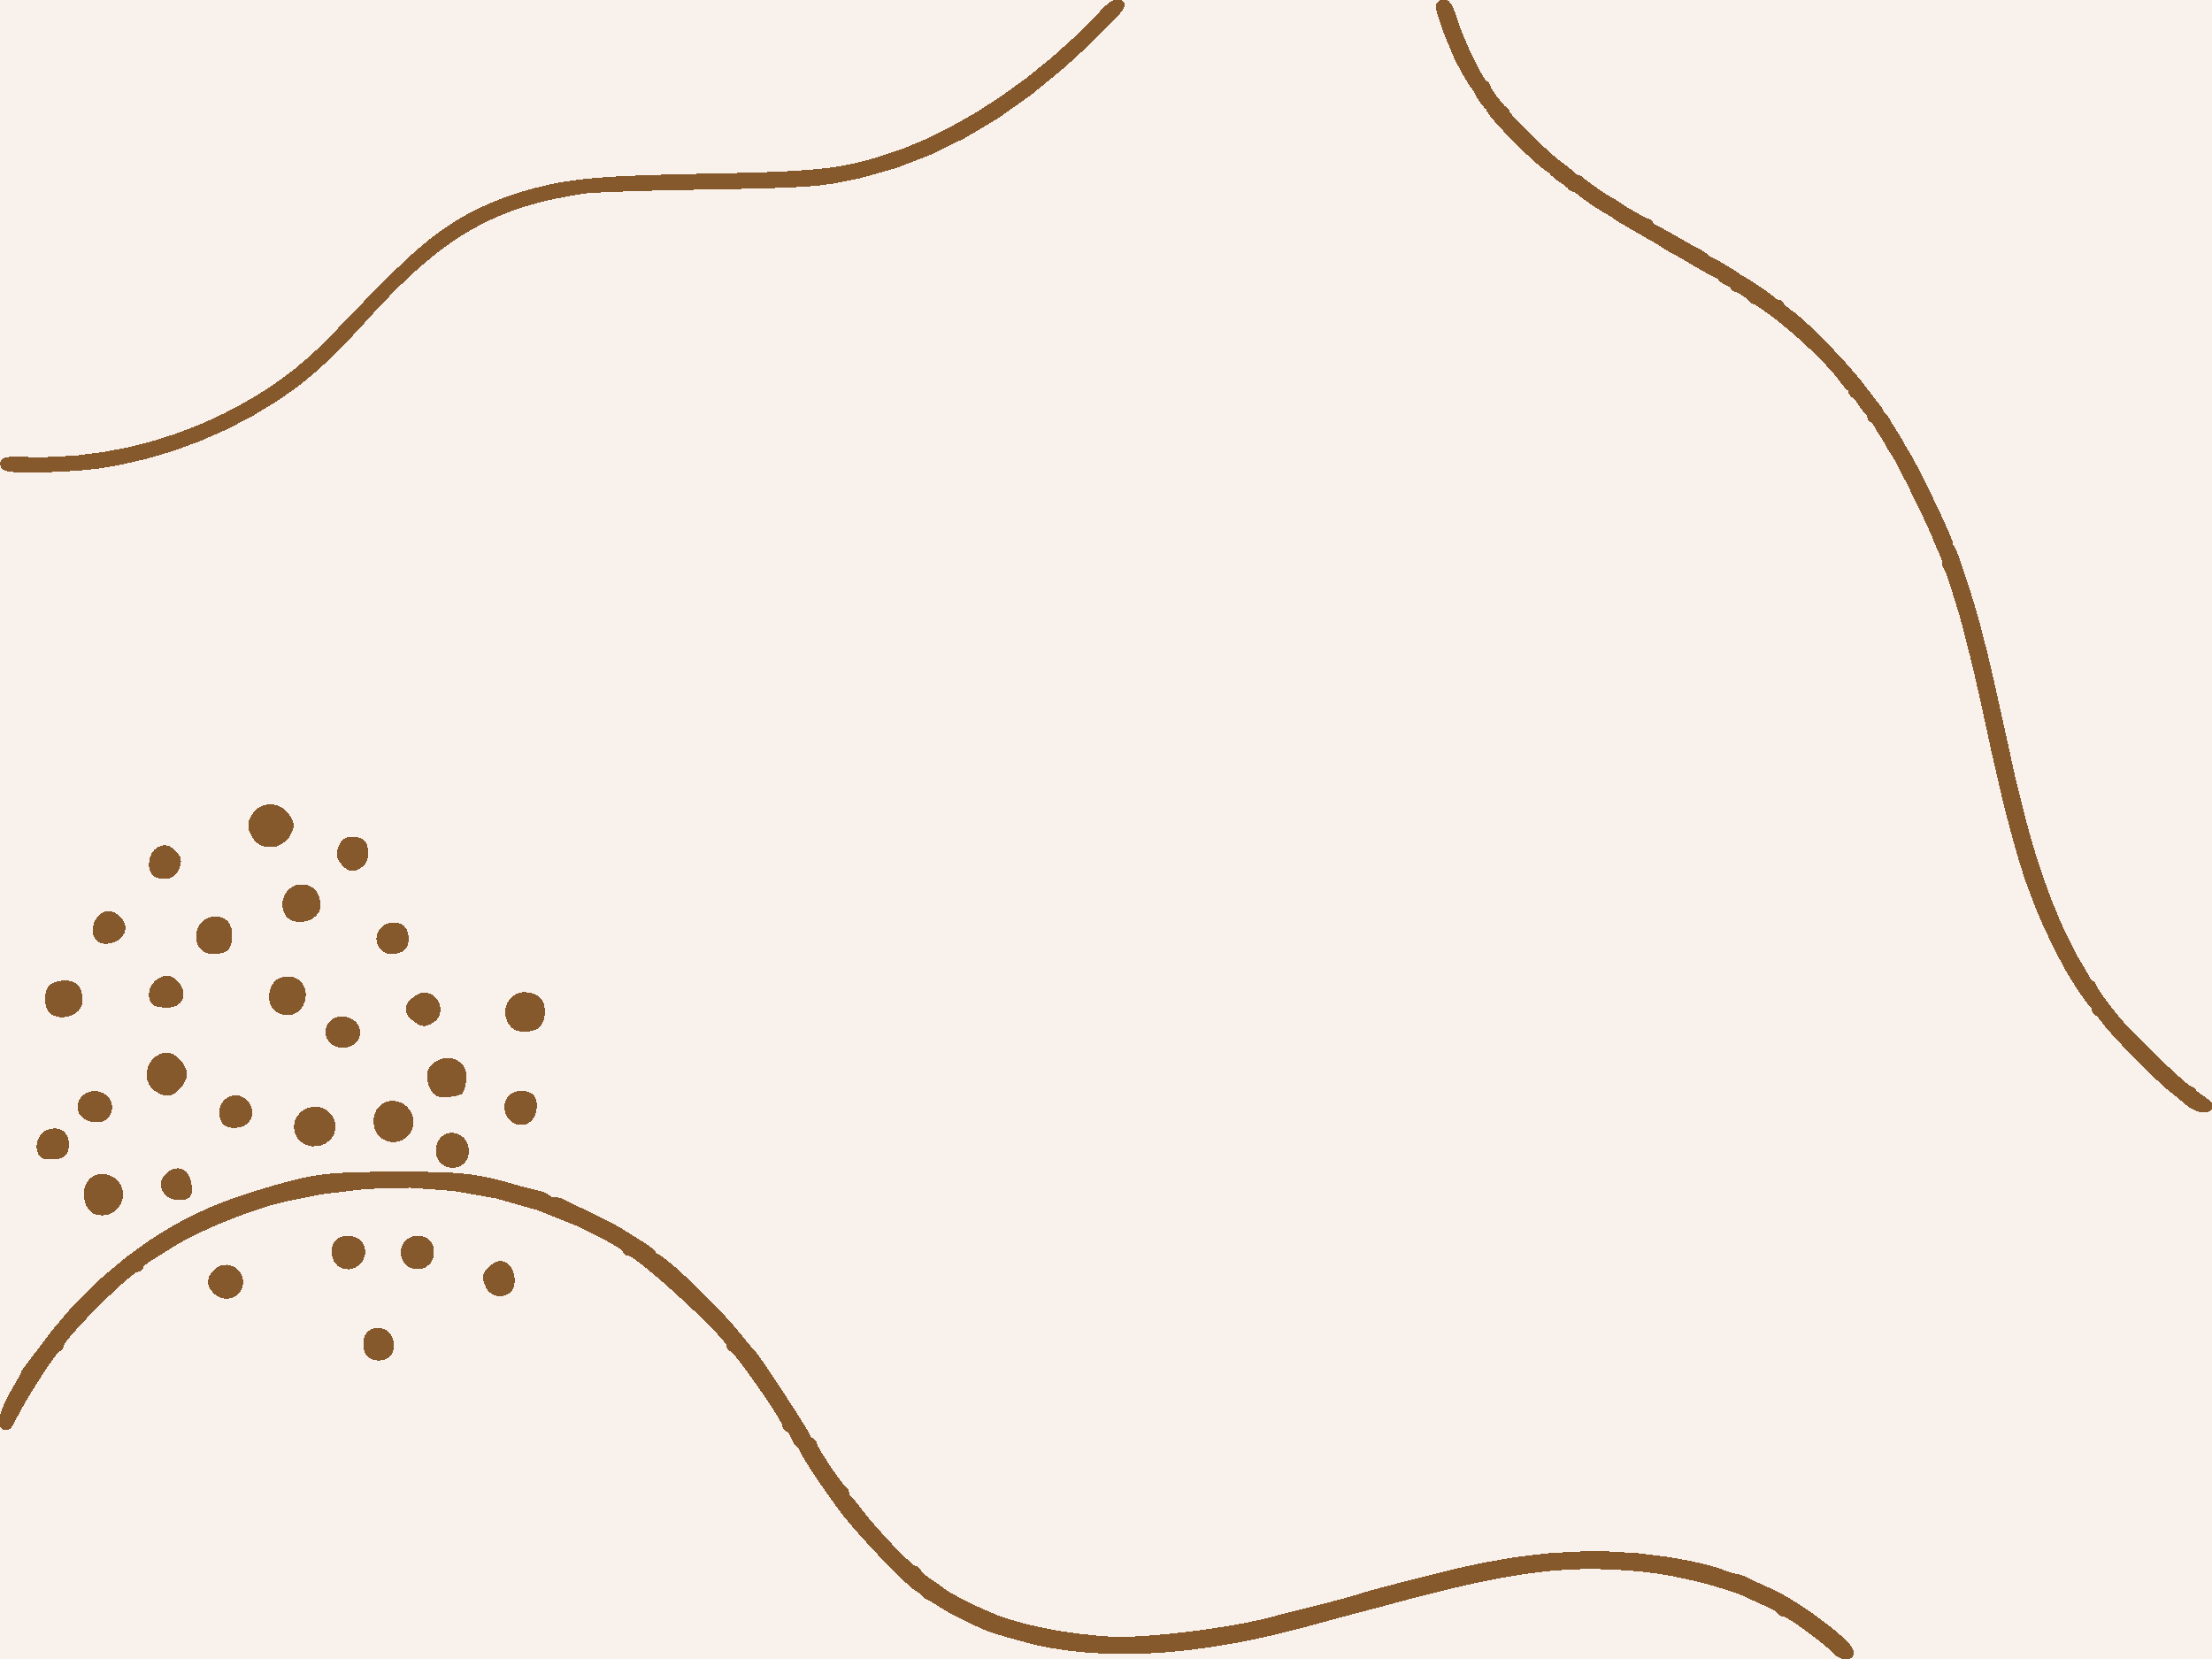
\includegraphics[width=\paperwidth,height=\paperheight]{images/assets/transition}}
\begin{frame}[noframenumbering]

\begin{center}
\Huge \textcolor{brown!70!black}{\textbf{Analytical}} \\
\Huge \textcolor{brown!70!black}{\textbf{gap equation}} \\
\Huge \textcolor{brown!70!black}{\textbf{accounting for}} \\
\Huge \textcolor{brown!70!black}{\textbf{Zeeman}}
\end{center}

\end{frame}}

%------------------------------------------------------------
\begin{frame}[noframenumbering]
\frametitle{Analytical gap equation accounting for Zeeman}

\begin{exampleblock}{Reparametrization of the onsite Hubbard self-energy}
\begin{equation*}
\boldsymbol{\Sigma}_{ii}=\left(\delta V_{\text{Z}}\left[\tau_{z}\otimes\sigma_{z}\right]-\delta\mu\left[\tau_{z}\otimes\sigma_{0}\right]\right)-\Delta\left[\tau_{y}\otimes\sigma_{y}\right]
\end{equation*}
\end{exampleblock}

\begin{columns}
\column{5cm}
\begin{alertblock}{Self-consistent pairing}
\vspace*{-4.5mm}
\begin{equation*}
-i\Delta\sigma_{y}=-U\left(\begin{array}{cc}
0 & \rho_{\uparrow\downarrow}^{\text{eh}}\\
\rho_{\downarrow\uparrow}^{\text{eh}} & 0
\end{array}\right)
\end{equation*}
\end{alertblock}

\column{6cm}
\begin{alertblock}{Induced magnetization and doping}
\vspace*{-4.5mm}
\begin{equation*}
-\delta V_{\text{Z}}\sigma_{z}-\delta\mu\sigma_{0}=-U\left(\begin{array}{cc}
\rho_{\downarrow\downarrow}^{\text{ee}} & 0\\
0 & \rho_{\uparrow\uparrow}^{\text{ee}}
\end{array}\right)
\end{equation*}
\end{alertblock}
\end{columns}
\pause

\begin{columns}
\column{1.5cm}
\column{9cm}
\begin{exampleblock}{}
\vspace*{-4.5mm}
\begin{align*}
&H(k)=\sum_{s}c_{ks}^{\dagger}\left[(\epsilon_{k}-\mu)\delta_{ss^{\prime}}+V_{Z}\sigma_{z}\right]c_{ks^{\prime}}\\\Rightarrow&\rho_{k\uparrow\downarrow}^{\text{eh}}=\frac{1}{N}\sum_{k}\left[u_{k+}^{*}v_{k+}f(\tilde{E}_{k+})+u_{k-}^{*}v_{k-}f(\tilde{E}_{k-})\right]
\end{align*}
\end{exampleblock}
\column{1.5cm}
\end{columns}

\begin{columns}
\column{4.5cm}
\begin{alertblock}{}
\vspace*{-4.5mm}
\begin{equation*}
\tilde{E}_{k\pm}=\tilde{V}_{\text{Z}}\pm\sqrt{\Delta^{2}+\tilde{\epsilon}_{k}^{2}}
\end{equation*}
\end{alertblock}

\column{3.5cm}
\begin{alertblock}{}
\vspace*{-5.5mm}
\begin{equation*}
\tilde{V}_{\text{Z}}=V_{\text{Z}}+\delta V_{\text{Z}}
\end{equation*}
\end{alertblock}

\column{2.5cm}
\begin{alertblock}{}
\vspace*{-6mm}
\begin{equation*}
\tilde{\epsilon}_{k}=\epsilon_{k}-\tilde{\mu}
\end{equation*}
\end{alertblock}
\end{columns}

\end{frame}

%------------------------------------------------------------
\begin{frame}[noframenumbering]
\frametitle{Analytical gap equation accounting for Zeeman}

\begin{block}{Self-consistent gap system of equations}
\begin{align*}
\Delta=&-U\sum_{k}\frac{\Delta}{4\tilde{E}_{k}}\left[\tanh\left(\frac{\tilde{V}_{\text{Z}}+\tilde{E}_{k}}{2k_{B}T}\right)-\tanh\left(\frac{\tilde{V}_{\text{Z}}-\tilde{E}_{k}}{2k_{B}T}\right)\right]\\&\\\delta V_{\text{Z}}=&-\frac{U}{2N}\sum_{k}\frac{\sinh\left(\frac{\tilde{V}_{Z}}{k_{B}T}\right)}{\cosh\left(\frac{\tilde{V}_{Z}}{k_{B}T}\right)+\cosh\left(\frac{\tilde{E}_{k}-\tilde{V}_{\text{Z}}}{k_{B}T}\right)}\\&\\\delta\mu=&\frac{U}{4}+\frac{U}{4N}\sum_{k}\frac{\tilde{\epsilon}_{k}}{2\tilde{E}_{k}}\left[\tanh\left(\frac{\tilde{V}_{\text{Z}}+\tilde{E}_{k}}{2k_{B}T}\right)-\tanh\left(\frac{\tilde{V}_{\text{Z}}-\tilde{E}_{k}}{2k_{B}T}\right)\right]
\end{align*}
\end{block}

\end{frame}

%------------------------------------------------------------
\begin{frame}[noframenumbering]
\frametitle{Analytical gap equation accounting for Zeeman}

\begin{exampleblock}{Conventional gap equation, $\Delta_{0}\equiv\Delta(V_{\text{Z}}=0)$}
\begin{equation*}
\Delta_{0}=-\frac{U}{N}\sum_{k}\frac{\Delta_{0}}{2E_{k}}\tanh\left(\frac{E_{k}}{2k_{B}T}\right),\text{ with }E_{k}=\sqrt{\Delta_{0}^{2}+\epsilon_{k}^{2}}
\end{equation*}
\end{exampleblock}
\pause

\begin{columns}
\column{3.5cm}
\begin{alertblock}{Dispersion}
\vspace*{-5mm}
\begin{equation*}
\epsilon_{k}\approx\pm v_{\text{F}}(k\mp k_{\text{F}})
\end{equation*}
\end{alertblock}

\column{5cm}
\begin{alertblock}{}
\vspace*{-4mm}
\begin{equation*}
\frac{1}{N}\sum_{k}\rightarrow\frac{a_{0}^{2}}{2\pi Lv_{F}}\int_{-\epsilon_{0}}^{\epsilon_{0}}dk
\end{equation*}
\end{alertblock}

\column{2.5cm}
\begin{alertblock}{}
\vspace*{-6mm}
\begin{equation*}
\Delta\ll\epsilon_{0}
\end{equation*}
\end{alertblock}
\vspace*{-2mm}

\begin{alertblock}{}
\vspace*{-6mm}
\begin{equation*}
U<0
\end{equation*}
\end{alertblock}
\end{columns}

\pause
\vspace*{0.25cm}
\begin{center}
\Large \textcolor{red!80!black}{---------$\ \bigstar$ \textbf{main result $\bigstar\ $}---------}
\end{center}

\begin{block}{Analytical gap equation accounting for Zeeman}
\vspace*{-4.5mm}
\begin{equation*}
\Delta=\frac{1}{2\epsilon_{0}}\sqrt{\Delta_{0}\left(2\left|V_{\text{Z}}\right|-\Delta_{0}\right)},\quad \Delta_{0}=2\epsilon_{0}\exp\left(-\sqrt{\frac{\pi^{2}}{2}\frac{\hbar^{2}}{m_{e}e}}\sqrt{\frac{\mu}{m_{0}}}\frac{1}{|U|a_{0}}\right)
\end{equation*}
\end{block}

\end{frame}

%------------------------------------------------------------
{\usebackgroundtemplate{
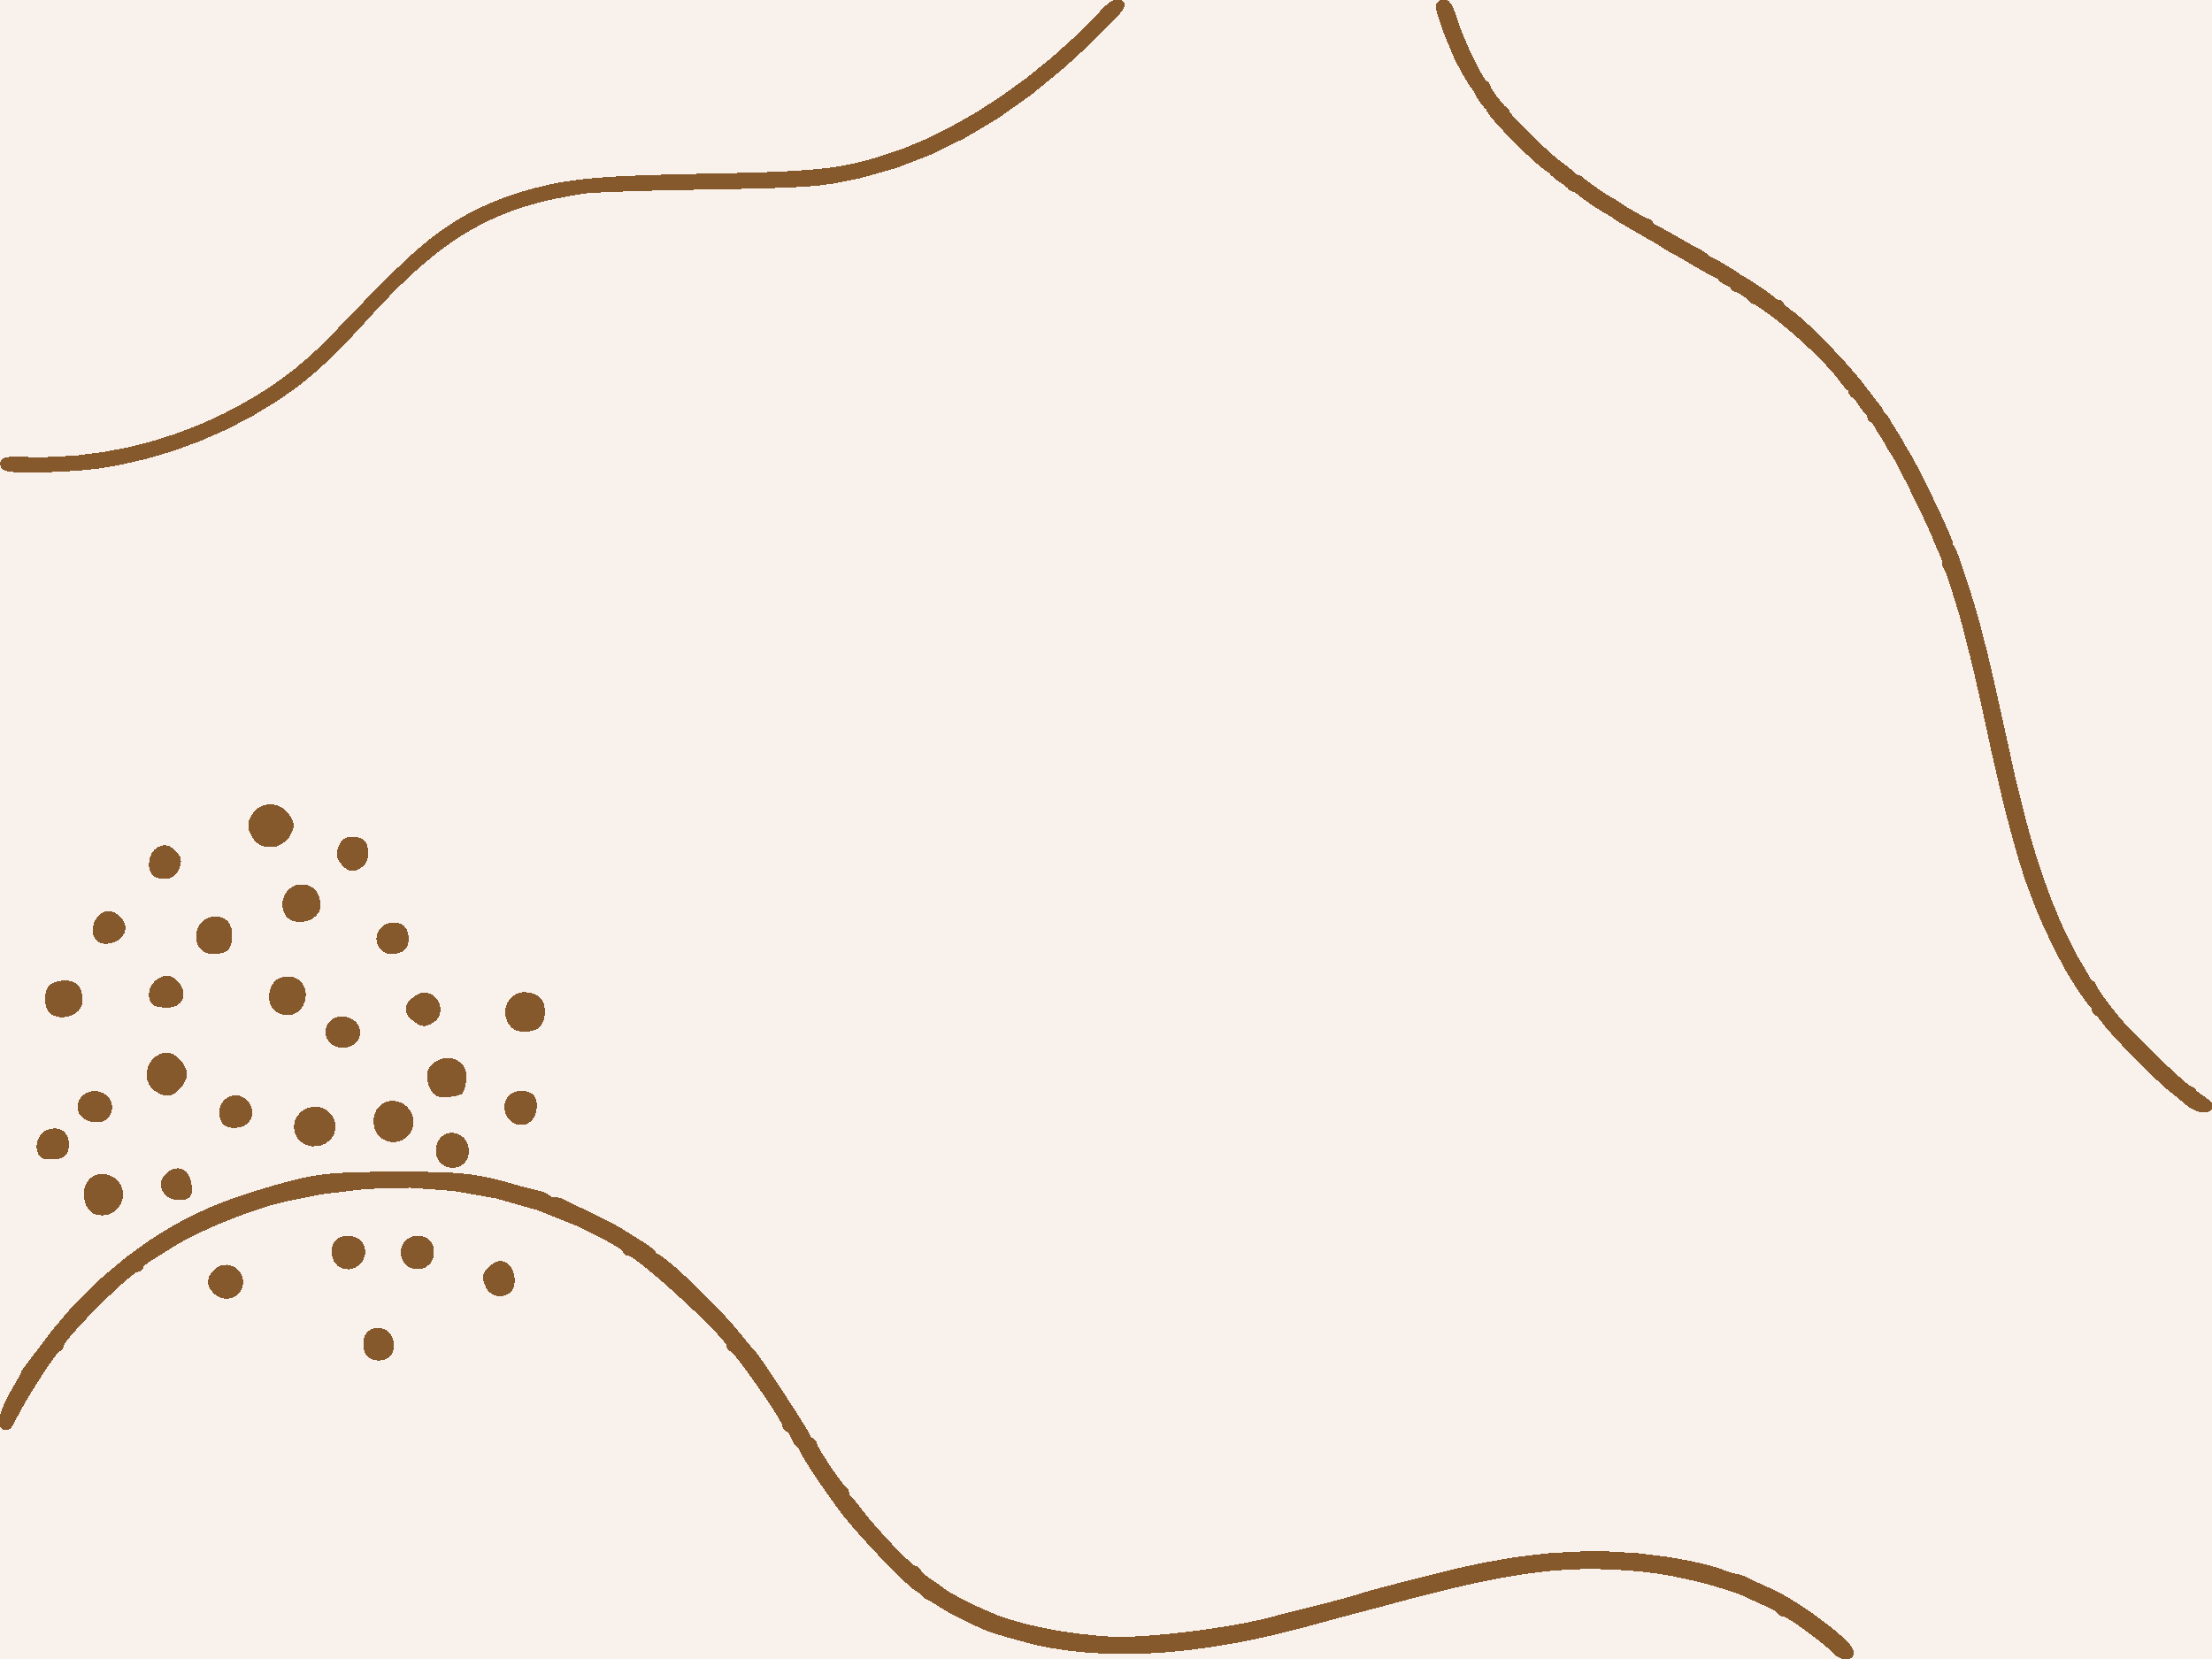
\includegraphics[width=\paperwidth,height=\paperheight]{images/assets/transition}}
\begin{frame}[noframenumbering]

\begin{center}
\Huge \textcolor{brown!70!black}{\textbf{Further}} \\
\Huge \textcolor{brown!70!black}{\textbf{details}}
\end{center}

\end{frame}}

%------------------------------------------------------------
\begin{frame}[noframenumbering]
\frametitle{Oreg-Lutchyn's Minimal Majorana model: \textcolor{black}{\underline{infinite length}}}

\begin{exampleblock}{}
\vspace*{-4mm}
\begin{equation*}
\hat{\boldsymbol{H}}=\sum_{\sigma_{i}\sigma_{j}}c_{\sigma_{i}}^{\dagger}\left(-\frac{\hbar^{2}}{2m^{*}}\partial_{x}^{2}-\mu-i\alpha_\text{R}\sigma_{y}\partial_{x}+V_{\text{Z}}\sigma_{x}\right)c_{\sigma_{j}}+\frac{1}{2}\left(\Delta_{0}c_{\uparrow}^{\dagger}c_{\downarrow}^{\dagger}+h.c\right)
\end{equation*}
\end{exampleblock}

\begin{center}
\begin{figure}
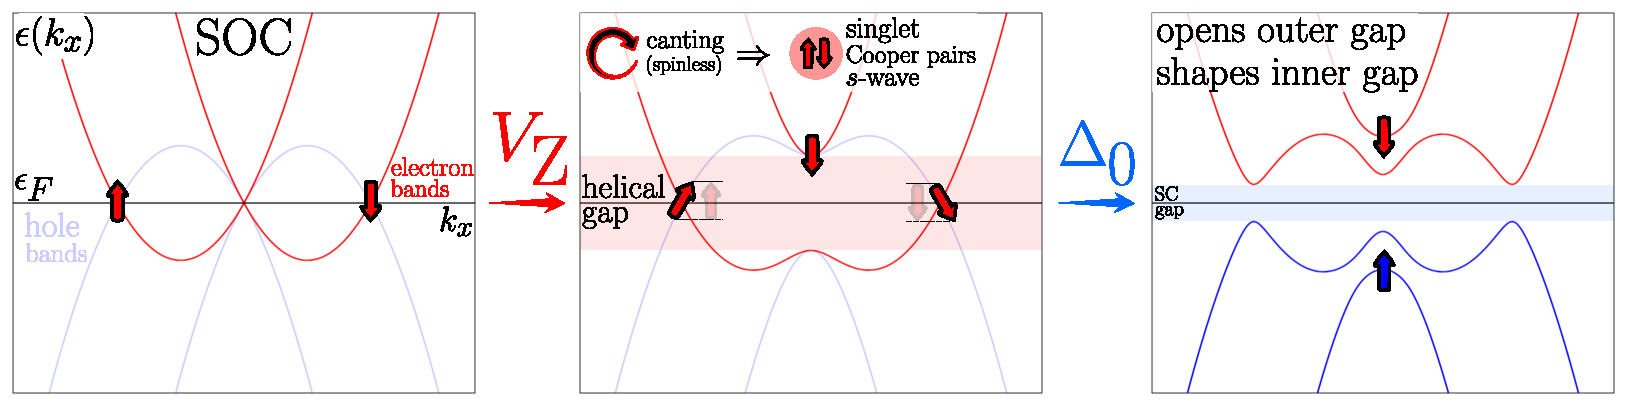
\includegraphics[scale=0.4]{images/lutchyn_bands}
\end{figure}
\end{center}
\pause

\begin{center}
\begin{figure}
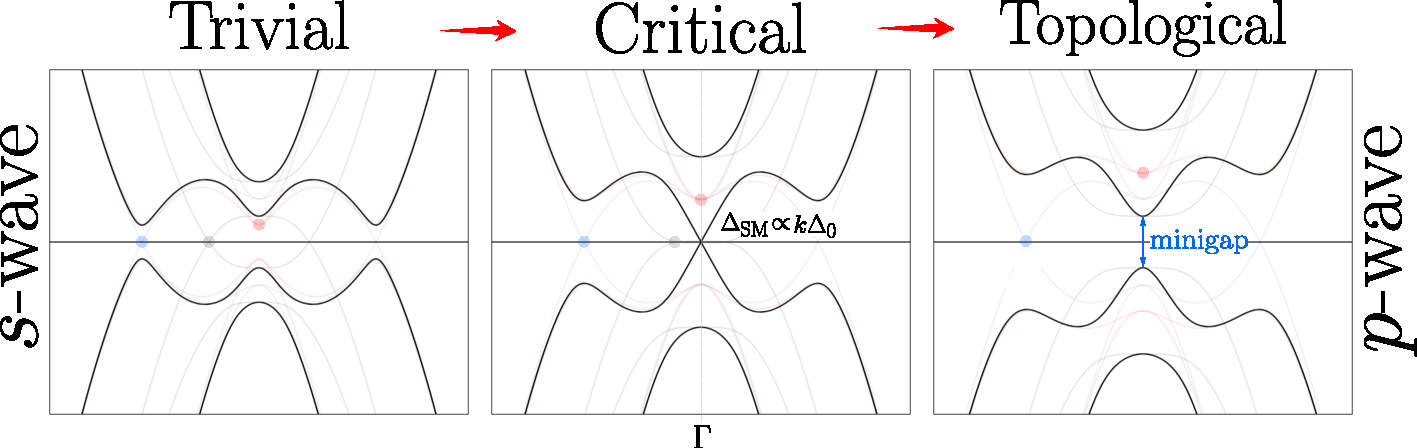
\includegraphics[scale=0.4]{images/lutchyn_phases}
\end{figure}
\end{center}

\end{frame}

%------------------------------------------------------------
\end{document}

